% !TEX program = xelatex
% 文件名:Main.tex
% 文件描述:四川大学网络空间安全学院2024研究生硕/博士 LaTeX 模版
% 作者:Yicheng Cai [xxx@gmail.com]
% 修改日期:2024年5月26日
 
% 设置文档属性
% 参数说明
% professional: 专业学位
% academic: 学术学位
% master: 硕士
% doctor: 博士
% approval: 送审版本,将不生成声明
% secret: 保密论文,将显示密级
% color: 红色川大logo
% kfont=<⟨none|adobe|fandol|founder|mac|macnew|macold|ubuntu|windows|windowsnew|windowsold|...⟩>,
% 不填写则默认fandol
% 送审和答辩用这个
\documentclass[approval,academic,master,34ch,caption-bi,kfont=windows]{../Template/scuthesis-cyc}
% 归档用这个
%\documentclass[academic,master,34ch,caption-bi,kfont=windows]{../Template/scuthesis-cyc}
\usepackage{pdfpages}  % 插入pdf文档
% 设置英文字体为Times New Roman
\usepackage{fontspec}
\setmainfont{Times New Roman}
\usepackage{amsmath}
\usepackage{amsfonts}
\usepackage{mathtools}
%\usepackage{algorithm}
%\usepackage[ruled,vlined]{algorithm2e} %很难用,且和algorithmic环境冲突
\usepackage{algorithmic}
%\usepackage{algpseudocode} %和algorithmic环境冲突
\captionsetup[algorithm]{font=small}
 % 如果希望彻底禁止某个浮动体的浮动效果,可以使用 float 宏包提供的 H 位置选项。 https://liam.page/2017/03/11/floats-in-LaTeX-basic/
\usepackage{float}

\usepackage{multirow}
\usepackage{booktabs}
\usepackage{hhline}
\usepackage{makecell}
\usepackage{diagbox}
\usepackage{lscape} % For landscape orientation
\usepackage{graphicx} % 用于插入图片
\usepackage{calc} % Needed for the \heightof command
\usepackage{colortbl} % 用于定义颜色
\usepackage{array}    % 用于表格布局
% 如何让表格部分横线加粗,改变表格线宽 https://www.latexstudio.net/archives/698.html
\makeatletter
\newcommand{\thickhline}{%
	\noalign {\ifnum 0=`}\fi \hrule height 1pt
	\futurelet \reserved@a \@xhline
}
\newcolumntype{"}{@{\hskip\tabcolsep\vrule width 1pt\hskip\tabcolsep}}
\makeatother

%https://zhuanlan.zhihu.com/p/488447829
\usepackage{longtable} % 引入长表格支持
%此命令用于调整续表标题的字号,这里默认为11号字体
%\renewcommand{\small}{\fontsize{11}{11}\selectfont}
\newcommand{\biaozihao}{\zihao{5}\rm\heiti}
\newcommand{\biaozihaoeng}{\zihao{5}\rm}

\usepackage{xcolor}   % 用于文本和背景颜色
\usepackage{subcaption}
\usepackage{epstopdf}
\usepackage{threeparttable}
\usepackage{colortbl}
\usepackage{pgf}

\newcommand*{\nicebar}[1]{\,\overline{#1}\,}

\definecolor{DarkRed}{RGB}{255, 180, 183}
\definecolor{LightRed}{RGB}{255, 232, 234}
\definecolor{DarkGreen}{RGB}{181, 224, 174}
\definecolor{LightGreen}{RGB}{231, 244, 228}
% 确保\newcommand在文档开始或任何文本内容之前定义
\newcommand{\colorForValue}[1]{%
	\pgfmathparse{int(#1< -0.12 ? 1 : (#1 < 0 ? 2 : (#1 < 0.12 ? 3 : 4)))}% 更正:添加int以确保结果为整数
	\ifcase\pgfmathresult\relax
	%	\or \cellcolor{red!30}% 浅红
	%	\or \cellcolor{red!15}% 淡红
	%	\or \cellcolor{green!15}% 淡绿
	%	\or \cellcolor{green!30}% 淡绿
	\or \cellcolor{DarkRed}% 浅绿
	\or \cellcolor{LightRed}% 浅绿
	\or \cellcolor{LightGreen}% 浅绿
	\or \cellcolor{DarkGreen}% 浅绿
	\fi
}

\begin{document}
	% 设置文档信息
	\unitid{10610} % 单位代码
	\STUnumber{202x2262400xx} % 学号或送审编号
	\securityClassification{秘密} % 密级:公开/内部/秘密/机密/绝密。当不使用secret时,不显示
	\securityYear{3} % 保密年限
	\CoverTitle{论文标题第一行} %封面标题
	\CoverSubTitle{论文标题第二行} %可做封面副标题
	\title{论文标题全称} % 论文全称
	\AbstractTitle{ 论文标题全称} %摘要标题
	%\ENGtitle{Research on Virtual Agent Identity Shaping and Personality Mimicking on Social Networks} %论文全称英文
	\ENGtitle{Full Thesis Title} %论文全称英文
	% \school{\zihao{5}{这里是特别长的单位名称甚至一行不能显示}} % 如果太长超出一行,可以根据显示效果修改字号,这里为5号字
	\school{四川大学网络空间安全学院} % 培养单位
	\ENGschool{School of Cyber Science and Engineering} % 培养单位英文
	\author{你的名字} % 作者姓名
	\ENGauthor{First Name Last Name} % 作者英文名
	\supervisor{贵导师} % 指导教师
	\ENGsupervisor{Prof. First Name Last Name} % 指导教师英文
	\degreeclass{学术硕士} % 学位类别
	\ENGdegreeclass{Master of Engineering} % 学位类别英文
	\major{网络空间安全} % 学科专业或领域名称
	\ENGmajor{Cybersecurity} % 学科专业或领域名称英文
	\hasmajor{1} % 若有领域则为1,否则改为0
	\defensedate{二〇二啥年啥月} % 论文答辩时间
	\grantdate{二〇二啥年啥月} % 学位授予时间
	\accomplishdate{二〇二啥年啥月} % 论文完成时间
	\statementdate{Month, 202x} % 声明时间
	\direction{查询录取方向}
	\ENGdirection{Information Content Security}
	\keywords{关键词 1$\quad$关键词 2$\quad$关键词 3$\quad$关键词 4$\quad$关键词 5}
	\ENGkeywords{Keyword one; Keyword two; Keyword three; Keyword four; Keyword five}
	
	% 自动制作封面
	\maketitle
	% 手动制作封面并插入
%	\includepdf[pages={1}]{封面-16开-优化.pdf}
%	\includepdf[pages={1}]{封面-16开-存档.pdf}
	% 自动制作中英文声明
	%	\makestatement
	% 设置论文正文前的页码、页眉等
	\frontmatter\pagenumbering{Roman}\pagestyle{fancy}
	% 包含摘要
	%!TEX root = ../Main.tex

% 中英文摘要
\begin{CHSabstract}
    好好想想怎么写

\end{CHSabstract}

\begin{ENGabstract}
Think more.
\end{ENGabstract}


	% 自动制作目录
	\maketoc
	% 自动制作图表目录
	\makefigtablist
	% 包含缩略词表
	%%!TEX root = ../Main.tex

% 常用缩略词表
\chapter{常用缩略词表}
\begin{appendix*}
\begin{tabular}{p{7em}p{25em}}
	Abbr. 1 & Abbreviation 1 \\
	Abbr. 2 & Abbreviation 2 \\
	Abbr. 3 & Abbreviation 3 \\
\end{tabular}
\end{appendix*}
	% 包含符号表
	%%!TEX root = ../Main.tex

% 常用符号表
\chapter{常用符号表}
\begin{appendix*}
	\begin{tabular}{p{7em}p{20em}}
		$Symbol_{1}$ & 符号$1$ \\
		$Symbol_{2}$ & 符号$2$ \\
		$Symbol_{3}$ & 符号$3$ \\
	\end{tabular}
\end{appendix*}
	% 设置论文正文部分的页码、页眉等
	\mainmatter\pagenumbering{arabic}\pagestyle{fancy}
	% 清除双数页 https://www.zhihu.com/question/266237548/answer/2691013672
	\let\cleardoublepage\clearpage
	% 包含第一章、第二章等等
	%!TEX root = ../Manual.tex
\chapter{前言}
\label{Chap_Intro}
本文档是《四川大学学位论文~\LaTeX~模版》的说明文档。


四川大学学位论文的工作以前由~dahakawang\footnote{\url{https://github.com/dahakawang/scu_thesis_template}}~、~tan\footnote{\url{http://www.codeforge.com/article/382397}}~等人做过。本模版是在参考~Casper Ti. Vector\footnote{\url{CasperVector@gmail.com}}~~\emph{pkuthss}~模版\cite{pkuthss}的基础上完成的。


Legendary L.\footnote{Legendary Leo \url{https://github.com/cuiao}}是本文档的创建者和维护者。

\section{特点}
\label{Sect_KeyFeatures}
本模版是严格按照《四川大学硕士、博士学位论文格式》\cite{SCUDissertationFormat}中的要求编写的,有以下几个特点:
\begin{itemize}
	\item 使用简单:本模版在编写之初就考虑到~\LaTeX~初学者的情况,按照本手册的说明,不需要高深的~\LaTeX~知识便可使用本模版进行论文写作。
	\item 自动化程度高:本模版的页码、标题、题注、目录等均使用了自动化命令,一般不需要用户干预。
	\item 写作方便:本模版的主要命令在样式文件中进行了封装,并采用了多文件编译方式。方便用户的写作与修改。
\end{itemize}

\section{推荐配置}
\label{Sect_RecommandedConfiguration}
本模版的使用和正确编译依赖以下几项:
\begin{description}[style=nextline,labelindent=2em,labelwidth=!]
	\item[中文字体] 本模版需要中文字体的支持。
	\item[\TeX~发行版] 一个支持中文的~\TeX~发行版,推荐使用~\TeX~Live\footnote{\url{https://www.tug.org/texlive/}}~,本模版即是使用~\TeX~Live~构建的。
	\item[文本编辑器] 一个好用的文本编辑器有利于你的写作,推荐使用~Atom\footnote{\url{https://atom.io/}}~,必备插件为~atom-latex\footnote{\url{https://github.com/thomasjo/atom-latex}}~和~language-latex\footnote{\url{https://github.com/area/language-latex}}~。
	\item[PDF~阅读器] 一个轻量级的~PDF~阅读器有利于提升效率,推荐使用~SumatraPDF\footnote{\url{http://www.sumatrapdfreader.org/free-pdf-reader.html}}~与~atom-latex~插件联用。
\end{description}


\section{模版文件}
\label{Sect_Files}
本模版根目录\verb|./|下文件夹或文件如下:
\dirtree{%
	.1 ../.
	.2 README.md\DTcomment{自述文件}.
	.2 Template\DTcomment{模版文件夹}.
	.2 MainBody\DTcomment{论文主体文件夹}.
	.2 Manual\DTcomment{手册(本文档)文件夹}.
}
其中,\verb|Template|(模版文件夹)较为重要,一般情况下请勿修改!以下按上述文件夹分类介绍本模版中的文件。

\subsection{模版文件夹}
\label{Subsect_TemplateFolder}
\verb|Template|为本模版最重要的文件夹,用于存放本模版的样式、宏定义、资源等文件,一般情况下请勿修改!详细的文件目录如下:
\dirtree{%
	.1 Template.
	.2 scuthesis.cls\DTcomment{模版样式文件}.
	.2 scuthesis.def\DTcomment{模版宏定义文件}.
	.2 chinesebst.bst\DTcomment{中文参考文献样式文件}.
	.2 Components.
	.3 Images.
	.4 SCU{\_}TITLE.eps\DTcomment{四川大学~LOGO}.
}

\subsection{论文主体文件夹}
\label{Subsect_MainbodyFolder}
\verb|MainBody|~文件夹主要用于填写论文内容,用户可以方便地将自己的论文按照章节填写到此文件夹中。详细的文件目录如下:
\dirtree{%
	.1 MainBody.
	.2 MainBody.tex\DTcomment{主\TeX文件}.
	.2 ReferenceBase.bib\DTcomment{参考文献库文件}.
	.2 Chapters\DTcomment{章节文件夹}.
	.3 0{\_}0{\_}Abstract.tex\DTcomment{中英文摘要}.
	.3 0{\_}1{\_}Abbreviations.tex\DTcomment{缩略词表}.
	.3 0{\_}2{\_}Symbols.tex\DTcomment{符号表}.
	.3 Introduction.tex\DTcomment{引言}.
	.3 Chapter2.tex\DTcomment{第二章}.
	.3 Thanks.tex\DTcomment{致谢}.
	.3 Achievements.tex\DTcomment{科研成果}.
	.3 CopyrightAuthorization.tex\DTcomment{版权授权(请勿修改)}.
	.3 OriginalStatement.tex\DTcomment{原创声明(请勿修改)}.
}
以上文件除~\verb|CopyrightAuthorization.tex|~和~\verb|OriginalStatement.tex|~按照学校统一的内容和格式规定禁止修改外,其他均可按照用户的需要进行修改。\\
\verb|ReferenceBase.bib|~可使用~\emph{EndNote\textsuperscript{\texttrademark}}~这类文献管理工具导出。


若~\verb|Chapters|~文件夹有改动,请使用~\verb|\include{Chapters/<文件名>}|~命令在~\verb|MainBody.tex|~做相应的修改(即若在~\verb|Chapters|~中增加了文件~\verb|Chapter3.tex|~,对应在~\verb|MainBody.tex|~的命令为~\verb|\include{Chapters/Chapter3}|~)。更多的使用方法请详见第\ref{Chap_UsingOfThisTemplate}章。

\subsection{手册文件夹}
\label{Subsect_ManualFolder}
\verb|Manual|~是本手册的文件夹,其内容与~\verb|MainBody|~较为类似,在此不做赘述。详细的文件目录如下:
\dirtree{%
	.1 Manual.
	.2 Manual.tex\DTcomment{本手册主\TeX文件}.
	.2 Manualbib.bib\DTcomment{本手册参考文献库文件}.
	.2 Manual.pdf\DTcomment{本手册}.
	.2 Chapters\DTcomment{本手册章节文件夹}.
	.3 0{\_}0{\_}Abstract.tex\DTcomment{中英文摘要}.
	.3 0{\_}1{\_}Abbreviations.tex\DTcomment{缩略词表}.
	.3 0{\_}2{\_}Symbols.tex\DTcomment{符号表}.
	.3 1{\_}Introduction.tex\DTcomment{前言(本章)}.
	.3 2{\_}Using.tex\DTcomment{模版的使用}.
	.3 3{\_}Realization.tex\DTcomment{部分功能实现}.
	.3 Thanks.tex\DTcomment{致谢}.
	.3 Achievements.tex\DTcomment{科研成果}.
	.3 CopyrightAuthorization.tex\DTcomment{版权授权(请勿修改)}.
	.3 OriginalStatement.tex\DTcomment{原创声明(请勿修改)}.
	.3 CopyrightStatement.tex\DTcomment{版权声明(请勿修改)}.
}

	%!TEX root = ../Main.tex

\chapter{相关技术介绍}
这章写多点哈
\section{引言}
本章将介绍xxx研究中涉及到的关键理论和技术,主要包括了xxx、xxx、xxx、xxx、xxx技术以及xxx技术。下面将对这些技术进行详细介绍。%下面将详细介绍各类技术的关键概念和相关原理。

\section{理论技术一}
\subsection{xxx}
迈尔斯-布里格斯类型指标(Myers-Briggs Type Indicator,简称MBTI)是一种深受欢迎且极具影响力的心理测评工具,它通过四个基本的二元维度——能量定向、信息获取、决策制定和生活方式——将个体分为十六种性格类型,每个类型代表了这些维度不同组合下的独特人格特征:
\begin{itemize}
	\item 能量定向:外倾(E)与内倾(I)
	\item 信息获取:实感(S)与直觉(N)
	\item 决策制定:思考(T)与情感(F)
	\item 生活方式:判断(J)与理解(P)
\end{itemize}

\section{统计学知识}
\subsection{斯皮尔曼相关系数}
斯皮尔曼相关系数(Spearman Correlation Coefficients)的计算方法如下:
	
\begin{enumerate}
	\item 为两个变量的每个观测值分配等级;
	\item 对每一对观测值,计算其等级差的平方,记为$D_i^2$;
	\item 计算所有$D_i^2$的和,记为$\sum D_i^2$;
	\item 使用以下公式计算斯皮尔曼相关系数$\rho$:
	 \begin{equation}
	 	\rho = 1 - \frac{6 \times \sum D_i^2}{n(n^2 - 1)}
	 \end{equation}
	其中,$n$是数据集中观测值的数量。
\end{enumerate}



\section{本章小结}
本章对xx所涉及的相关技术进行了详细的描述。首先介绍了xx。其次,介绍了xxx。最后,本章对xx做了必要的介绍。



	%!TEX root = ../Main.tex

\chapter{研究一}\label{ch-name}
\section{引言}

\section{模块一}\label{sec-feature}

\subsection{子模块}

详见表格\ref{tab:name}

\begin{table}[htbp]\footnotesize
	\bicaption{图xx征}{Ixatures}
	\label{tab:name}
    \begin{tabular}{p{1cm}llp{9.3cm}}
		\hline
		\rowcolor{gray!15}
		\textbf{类别}                   & \textbf{特征}             & \textbf{维度} & \textbf{概述}                                              \\ \hline
		\multirow{4}{*}{颜色}              & HSxx          & 5          & H通道xx准差 \\
		& 颜色xx             & 3          & Valxx量                           \\
		& 颜xx          & 1          & 到均一xxe,xx)                                                                                    \\
		& 颜色xx例                & 11         & 黑色xx色和黄色的占比                                                \\
		\hline
		\multirow{4}{*}{xxx图}        & xx素               & 1          & Caxx素的比例                           \\
		& 细xxx           & 2          & Meaxx率                                                                              \\
		& 浅xx标  & 3          & 图像xx度                                            \\
		& 三xx则            & 2          & 图像xx                                                  \\
		\hline
		\multirow{5}{*}{纹xx} & xxx & 1          & 图xx熵                                                           \\
		& xx理    & 12         & 通过Daubss度水平                                     \\
		& xx纹理                    & 3          & 粗xx方向性的量                                            \\
		& Gxx理           & 12         & 每个Hxx匀性的量                                       \\
		 & GIxx理          & 24         & 用于xx输出                                       \\ 
		\hline
		% \cline{2-4} 
	\end{tabular}
\end{table}
\vspace{-10pt}

具体流程见算法\ref{alg:name}。

\begin{algorithm}\small
	\caption{计xx类别比例}\label{alg:name}
	\begin{algorithmic}[1]
		\REQUIRE 图像,存储在\texttt{bgr\_img}中;颜色xx,存储在\texttt{"color\_dict.npz"}中
		\ENSURE 图像中每xx分比列表
		
		\STATE // 统计xx次
		\STATE 加xx典\texttt{"color\_dict.npz"}至\texttt{color\_dict}
		\STATE 将\texttt{bgr\_img}从xx格式
		\STATE 将Rxx除以8
		\STATE 将xxxx通道
		\STATE 对于每个像素,计算唯一键:\texttt{unique\_key = red * (32 * 32) + green * 32 + blue}
		\STATE // 计算图xx分比
		\STATE 使用\texttt{unique\_key}从\texttt{color\_dict}中xx频率
		\STATE 计算xx度(\texttt{h})和宽度(\texttt{w})
		\STATE 对图xx,并除以h·w
		\STATE 返回xx列表
	\end{algorithmic}
\end{algorithm}


\begin{table}[h!]\small%[htbp]\small
	\centering
	\begin{threeparttable}[b]
		\bicaption{人脸x表}{InventoryxMBTxality}
		\label{tbl:dataset survey}
		\begin{tabular}{|c|p{7.4cm}|p{5cm}|} 
			\hline
			\rowcolor{gray!15}
			序号 & 原xx题 & 问题翻译 \\
			\hline
			1 & Pleasxxe. & 请上传一xx活照。 \\  
			\hline
			2 & Please xxe test\tnote{*} and uploadxxt result. & 请做xx果截图。\\
			\hline  
			3 & Please select your pxxnt test. & 请根据xx类型.\\
			\hline
			4 & Is the resxxicable". & 本次测xx合”。\\  
			\hline
		\end{tabular}
		\begin{tablenotes}
			\footnotesize
			\item[*] 16perxersonality-test。
		\end{tablenotes}
	\end{threeparttable}
\end{table}



\begin{table}[ht]\footnotesize
	\centering
	\bicaption{Mxx计信息}{MBxxtistics}
	\label{tbl:text-dataset-stats}
	\begin{tabular}{c|c||ccc}
		\hline%\toprule
		\rowcolor{gray!15}
		数据集 & 人xx质 & 训练集 (60\%) & 验证集 (20\%) & 测试集 (20\%) \\
		\hline%\midrule
		\multirow{4}{*}{Mxxk} & xx & 4x8 / 11x2 & 14x/ 38x6 & 143x7 / x77 \\
		& xx & 7xx / 48xx& x / 1x5 & 2x/ 16x\\
		& xx & 3xx9 / 1xx1 & 11xx0 / 6x3 & 11x2 / x2 \\
		& xx & 3xx1 / 2xx9 & 10x3 / x0 & x6 / 7x8 \\
		\hline%\addlinespace
		\multirow{4}{*}{Kaxe} & x & 40x/ 1x4 & 1x6 / 4x & 1x9 / x6 \\
		& x & 6x/ 4478 & x2 / x & x8 / 1x\\
		& x & 24x0 / 2x95 & 7x1 / 9x4 & 78x/ x5 \\
		& Jx & 3x96 / 2x09 & 10x3 / x2 & 10x / x3 \\
		\hline%\bottomrule
	\end{tabular}
\end{table}




\vspace{20pt}

\begin{footnotesize}
\begin{longtable}{|l||c|c|c|c|c||c|c|c|c|}
	\bicaption{视觉x系数}{Spexsoxraits}
	\label{tab:xon}\\%这里的换行符号一定要有!!!去掉会报错的
	
	% 首页的表头
	\hline%	\thickhline
	\rowcolor{gray!15} \textbf{特征} & \multicolumn{5}{c||}{\textbf{大x格}} & \multicolumn{4}{c|}{\textbf{Mx}} \\

%	\hline%\thickhline
	\hhline{*{10}{:=}:}%\thickhline
	\rowcolor{gray!15} \textbf{颜色} & \textbf{Ox} & \textbf{Cxn} & \textbf{x} & \textbf{xr} & \textbf{xu} & \textbf{I} & \textbf{N} & \textbf{F} & \textbf{J} \\
	\hhline{*{10}{:=}:}%\thickhline
	
	\endfirsthead
	
	%续表的表头
	
	%此命令用于控制续表标题的上行距
	\specialrule{0em}{0pt}{-8pt}%{8pt}%{11.06pt}
	
	\multicolumn{10}{c}{\biaozihao 续表 \ref{tab:xon}\ \ \ \ 视觉x与x数\vspace{5pt}}\\	
	\multicolumn{10}{c}{\biaozihaoeng Table \ref{tab:xon}\ \ \ \ Spxts }\\%(continued)}\\	
	
	%此命令用于控制续表标题的下行距
	\specialrule{0em}{0pt}{5pt}%{5.03pt}
	
	% 续表的表头具体内容
	
	\hline%\thickhline
	\rowcolor{gray!15} \textbf{特征} & \multicolumn{5}{c||}{\textbf{x人格}} & \multicolumn{4}{c|}{\textbf{xI}} \\

	\hhline{*{10}{:=}:}%\thickhline
	\rowcolor{gray!15} \textbf{x理} & \textbf{Ox} & \textbf{xon} & \textbf{Ex} & \textbf{xr} & \textbf{Nx} & \textbf{E} & \textbf{N} & \textbf{F} & \textbf{P} \\
	\hline%\thickhline
	
	\endhead
	
	% 表底
	\hline%\thickhline
	\endfoot
	
	\hline%\thickhline
	\endlastfoot
	\hline
	色x(H) & \colorForValue{-0.203} -0.203 & \colorForValue{-0.15} -0.15 & \colorForValue{0.077} 0.077 & \colorForValue{-0.068} -0.068 & \colorForValue{0.537} 0.537 & \colorForValue{-0.038} -0.038 & \colorForValue{-0.032} -0.032 & \colorForValue{-0.073} -0.073 & \colorForValue{-0.061} -0.061 \\
	\hline
	色x(H) & \colorForValue{-0.203} -0.203 & \colorForValue{-0.15} -0.15 & \colorForValue{0.077} 0.077 & \colorForValue{-0.068} -0.068 & \colorForValue{0.537} 0.537 & \colorForValue{-0.038} -0.038 & \colorForValue{-0.032} -0.032 & \colorForValue{-0.073} -0.073 & \colorForValue{-0.061} -0.061 \\
	\hline
	色x(H) & \colorForValue{-0.203} -0.203 & \colorForValue{-0.15} -0.15 & \colorForValue{0.077} 0.077 & \colorForValue{-0.068} -0.068 & \colorForValue{0.537} 0.537 & \colorForValue{-0.038} -0.038 & \colorForValue{-0.032} -0.032 & \colorForValue{-0.073} -0.073 & \colorForValue{-0.061} -0.061 \\
	\hline
	色x(H) & \colorForValue{-0.203} -0.203 & \colorForValue{-0.15} -0.15 & \colorForValue{0.077} 0.077 & \colorForValue{-0.068} -0.068 & \colorForValue{0.537} 0.537 & \colorForValue{-0.038} -0.038 & \colorForValue{-0.032} -0.032 & \colorForValue{-0.073} -0.073 & \colorForValue{-0.061} -0.061 \\
	\hline
	色x(H) & \colorForValue{-0.203} -0.203 & \colorForValue{-0.15} -0.15 & \colorForValue{0.077} 0.077 & \colorForValue{-0.068} -0.068 & \colorForValue{0.537} 0.537 & \colorForValue{-0.038} -0.038 & \colorForValue{-0.032} -0.032 & \colorForValue{-0.073} -0.073 & \colorForValue{-0.061} -0.061 \\
	\hline
	色x(H) & \colorForValue{-0.203} -0.203 & \colorForValue{-0.15} -0.15 & \colorForValue{0.077} 0.077 & \colorForValue{-0.068} -0.068 & \colorForValue{0.537} 0.537 & \colorForValue{-0.038} -0.038 & \colorForValue{-0.032} -0.032 & \colorForValue{-0.073} -0.073 & \colorForValue{-0.061} -0.061 \\
	\hline
	色x(H) & \colorForValue{-0.203} -0.203 & \colorForValue{-0.15} -0.15 & \colorForValue{0.077} 0.077 & \colorForValue{-0.068} -0.068 & \colorForValue{0.537} 0.537 & \colorForValue{-0.038} -0.038 & \colorForValue{-0.032} -0.032 & \colorForValue{-0.073} -0.073 & \colorForValue{-0.061} -0.061 \\
	\hline
	色x(H) & \colorForValue{-0.203} -0.203 & \colorForValue{-0.15} -0.15 & \colorForValue{0.077} 0.077 & \colorForValue{-0.068} -0.068 & \colorForValue{0.537} 0.537 & \colorForValue{-0.038} -0.038 & \colorForValue{-0.032} -0.032 & \colorForValue{-0.073} -0.073 & \colorForValue{-0.061} -0.061 \\
	\hline
	色x(H) & \colorForValue{-0.203} -0.203 & \colorForValue{-0.15} -0.15 & \colorForValue{0.077} 0.077 & \colorForValue{-0.068} -0.068 & \colorForValue{0.537} 0.537 & \colorForValue{-0.038} -0.038 & \colorForValue{-0.032} -0.032 & \colorForValue{-0.073} -0.073 & \colorForValue{-0.061} -0.061 \\
	\hline
	色x(H) & \colorForValue{-0.203} -0.203 & \colorForValue{-0.15} -0.15 & \colorForValue{0.077} 0.077 & \colorForValue{-0.068} -0.068 & \colorForValue{0.537} 0.537 & \colorForValue{-0.038} -0.038 & \colorForValue{-0.032} -0.032 & \colorForValue{-0.073} -0.073 & \colorForValue{-0.061} -0.061 \\
	\hline
	色x(H) & \colorForValue{-0.203} -0.203 & \colorForValue{-0.15} -0.15 & \colorForValue{0.077} 0.077 & \colorForValue{-0.068} -0.068 & \colorForValue{0.537} 0.537 & \colorForValue{-0.038} -0.038 & \colorForValue{-0.032} -0.032 & \colorForValue{-0.073} -0.073 & \colorForValue{-0.061} -0.061 \\
	\hline
	色x(H) & \colorForValue{-0.203} -0.203 & \colorForValue{-0.15} -0.15 & \colorForValue{0.077} 0.077 & \colorForValue{-0.068} -0.068 & \colorForValue{0.537} 0.537 & \colorForValue{-0.038} -0.038 & \colorForValue{-0.032} -0.032 & \colorForValue{-0.073} -0.073 & \colorForValue{-0.061} -0.061 \\
	\hline
	色x(H) & \colorForValue{-0.203} -0.203 & \colorForValue{-0.15} -0.15 & \colorForValue{0.077} 0.077 & \colorForValue{-0.068} -0.068 & \colorForValue{0.537} 0.537 & \colorForValue{-0.038} -0.038 & \colorForValue{-0.032} -0.032 & \colorForValue{-0.073} -0.073 & \colorForValue{-0.061} -0.061 \\
	\hline
	色x(H) & \colorForValue{-0.203} -0.203 & \colorForValue{-0.15} -0.15 & \colorForValue{0.077} 0.077 & \colorForValue{-0.068} -0.068 & \colorForValue{0.537} 0.537 & \colorForValue{-0.038} -0.038 & \colorForValue{-0.032} -0.032 & \colorForValue{-0.073} -0.073 & \colorForValue{-0.061} -0.061 \\
	\hline
	色x(H) & \colorForValue{-0.203} -0.203 & \colorForValue{-0.15} -0.15 & \colorForValue{0.077} 0.077 & \colorForValue{-0.068} -0.068 & \colorForValue{0.537} 0.537 & \colorForValue{-0.038} -0.038 & \colorForValue{-0.032} -0.032 & \colorForValue{-0.073} -0.073 & \colorForValue{-0.061} -0.061 \\
	\hline
	色x(H) & \colorForValue{-0.203} -0.203 & \colorForValue{-0.15} -0.15 & \colorForValue{0.077} 0.077 & \colorForValue{-0.068} -0.068 & \colorForValue{0.537} 0.537 & \colorForValue{-0.038} -0.038 & \colorForValue{-0.032} -0.032 & \colorForValue{-0.073} -0.073 & \colorForValue{-0.061} -0.061 \\
	\hline
	色x(H) & \colorForValue{-0.203} -0.203 & \colorForValue{-0.15} -0.15 & \colorForValue{0.077} 0.077 & \colorForValue{-0.068} -0.068 & \colorForValue{0.537} 0.537 & \colorForValue{-0.038} -0.038 & \colorForValue{-0.032} -0.032 & \colorForValue{-0.073} -0.073 & \colorForValue{-0.061} -0.061 \\
	\hline
	色x(H) & \colorForValue{-0.203} -0.203 & \colorForValue{-0.15} -0.15 & \colorForValue{0.077} 0.077 & \colorForValue{-0.068} -0.068 & \colorForValue{0.537} 0.537 & \colorForValue{-0.038} -0.038 & \colorForValue{-0.032} -0.032 & \colorForValue{-0.073} -0.073 & \colorForValue{-0.061} -0.061 \\
	\hline
	色x(H) & \colorForValue{-0.203} -0.203 & \colorForValue{-0.15} -0.15 & \colorForValue{0.077} 0.077 & \colorForValue{-0.068} -0.068 & \colorForValue{0.537} 0.537 & \colorForValue{-0.038} -0.038 & \colorForValue{-0.032} -0.032 & \colorForValue{-0.073} -0.073 & \colorForValue{-0.061} -0.061 \\
	\hline
	色x(H) & \colorForValue{-0.203} -0.203 & \colorForValue{-0.15} -0.15 & \colorForValue{0.077} 0.077 & \colorForValue{-0.068} -0.068 & \colorForValue{0.537} 0.537 & \colorForValue{-0.038} -0.038 & \colorForValue{-0.032} -0.032 & \colorForValue{-0.073} -0.073 & \colorForValue{-0.061} -0.061 \\
	\hhline{*{10}{:=}:}%\thickhline
	\rowcolor{gray!15} \textbf{构x} & \textbf{Ope} & \textbf{Con} & \textbf{Ext} & \textbf{Agr} & \textbf{Neu} & \textbf{I} & \textbf{N} & \textbf{T} & \textbf{J} \\
	\hhline{*{10}{:=}:}%\thickhline
	边x & \colorForValue{-0.371} -0.371 & \colorForValue{0.127} 0.127 & \colorForValue{-0.414} -0.414 & \colorForValue{0.383} 0.383 & \colorForValue{0.338} 0.338 & \colorForValue{0.076} 0.076 & \colorForValue{-0.102} -0.102 & \colorForValue{-0.474} -0.474 & \colorForValue{-0.227} -0.227 \\
	\hline
	边x & \colorForValue{-0.371} -0.371 & \colorForValue{0.127} 0.127 & \colorForValue{-0.414} -0.414 & \colorForValue{0.383} 0.383 & \colorForValue{0.338} 0.338 & \colorForValue{0.076} 0.076 & \colorForValue{-0.102} -0.102 & \colorForValue{-0.474} -0.474 & \colorForValue{-0.227} -0.227 \\
	\hline
	边x & \colorForValue{-0.371} -0.371 & \colorForValue{0.127} 0.127 & \colorForValue{-0.414} -0.414 & \colorForValue{0.383} 0.383 & \colorForValue{0.338} 0.338 & \colorForValue{0.076} 0.076 & \colorForValue{-0.102} -0.102 & \colorForValue{-0.474} -0.474 & \colorForValue{-0.227} -0.227 \\
	\hline
	边x & \colorForValue{-0.371} -0.371 & \colorForValue{0.127} 0.127 & \colorForValue{-0.414} -0.414 & \colorForValue{0.383} 0.383 & \colorForValue{0.338} 0.338 & \colorForValue{0.076} 0.076 & \colorForValue{-0.102} -0.102 & \colorForValue{-0.474} -0.474 & \colorForValue{-0.227} -0.227 \\
	\hline
	边x & \colorForValue{-0.371} -0.371 & \colorForValue{0.127} 0.127 & \colorForValue{-0.414} -0.414 & \colorForValue{0.383} 0.383 & \colorForValue{0.338} 0.338 & \colorForValue{0.076} 0.076 & \colorForValue{-0.102} -0.102 & \colorForValue{-0.474} -0.474 & \colorForValue{-0.227} -0.227 \\
	\hline
	边x & \colorForValue{-0.371} -0.371 & \colorForValue{0.127} 0.127 & \colorForValue{-0.414} -0.414 & \colorForValue{0.383} 0.383 & \colorForValue{0.338} 0.338 & \colorForValue{0.076} 0.076 & \colorForValue{-0.102} -0.102 & \colorForValue{-0.474} -0.474 & \colorForValue{-0.227} -0.227 \\
	\hline
	边x & \colorForValue{-0.371} -0.371 & \colorForValue{0.127} 0.127 & \colorForValue{-0.414} -0.414 & \colorForValue{0.383} 0.383 & \colorForValue{0.338} 0.338 & \colorForValue{0.076} 0.076 & \colorForValue{-0.102} -0.102 & \colorForValue{-0.474} -0.474 & \colorForValue{-0.227} -0.227 \\
	\hline
	边x & \colorForValue{-0.371} -0.371 & \colorForValue{0.127} 0.127 & \colorForValue{-0.414} -0.414 & \colorForValue{0.383} 0.383 & \colorForValue{0.338} 0.338 & \colorForValue{0.076} 0.076 & \colorForValue{-0.102} -0.102 & \colorForValue{-0.474} -0.474 & \colorForValue{-0.227} -0.227 \\
	\hhline{*{10}{:=}:}%\thickhline
	\rowcolor{gray!15} \textbf{xxx} & \textbf{Ope} & \textbf{Con} & \textbf{Ext} & \textbf{Agr} & \textbf{Neu} & \textbf{I} & \textbf{N} & \textbf{T} & \textbf{J} \\
	\hhline{*{10}{:=}:}%\thickhline
	x熵 & \colorForValue{-0.346} -0.346 & \colorForValue{0.498} 0.498 & \colorForValue{0.206} 0.206 & \colorForValue{-0.313} -0.313 & \colorForValue{0.492} 0.492 & \colorForValue{0.254} 0.254 & \colorForValue{-0.071} -0.071 & \colorForValue{-0.315} -0.315 & \colorForValue{-0.037} -0.037 \\
	\hline
	x熵 & \colorForValue{-0.346} -0.346 & \colorForValue{0.498} 0.498 & \colorForValue{0.206} 0.206 & \colorForValue{-0.313} -0.313 & \colorForValue{0.492} 0.492 & \colorForValue{0.254} 0.254 & \colorForValue{-0.071} -0.071 & \colorForValue{-0.315} -0.315 & \colorForValue{-0.037} -0.037 \\
	\hline
	x熵 & \colorForValue{-0.346} -0.346 & \colorForValue{0.498} 0.498 & \colorForValue{0.206} 0.206 & \colorForValue{-0.313} -0.313 & \colorForValue{0.492} 0.492 & \colorForValue{0.254} 0.254 & \colorForValue{-0.071} -0.071 & \colorForValue{-0.315} -0.315 & \colorForValue{-0.037} -0.037 \\
	\hline
	x熵 & \colorForValue{-0.346} -0.346 & \colorForValue{0.498} 0.498 & \colorForValue{0.206} 0.206 & \colorForValue{-0.313} -0.313 & \colorForValue{0.492} 0.492 & \colorForValue{0.254} 0.254 & \colorForValue{-0.071} -0.071 & \colorForValue{-0.315} -0.315 & \colorForValue{-0.037} -0.037 \\
	\hline
	x熵 & \colorForValue{-0.346} -0.346 & \colorForValue{0.498} 0.498 & \colorForValue{0.206} 0.206 & \colorForValue{-0.313} -0.313 & \colorForValue{0.492} 0.492 & \colorForValue{0.254} 0.254 & \colorForValue{-0.071} -0.071 & \colorForValue{-0.315} -0.315 & \colorForValue{-0.037} -0.037 \\
	\hline
	x熵 & \colorForValue{-0.346} -0.346 & \colorForValue{0.498} 0.498 & \colorForValue{0.206} 0.206 & \colorForValue{-0.313} -0.313 & \colorForValue{0.492} 0.492 & \colorForValue{0.254} 0.254 & \colorForValue{-0.071} -0.071 & \colorForValue{-0.315} -0.315 & \colorForValue{-0.037} -0.037 \\
	\hline
	x熵 & \colorForValue{-0.346} -0.346 & \colorForValue{0.498} 0.498 & \colorForValue{0.206} 0.206 & \colorForValue{-0.313} -0.313 & \colorForValue{0.492} 0.492 & \colorForValue{0.254} 0.254 & \colorForValue{-0.071} -0.071 & \colorForValue{-0.315} -0.315 & \colorForValue{-0.037} -0.037 \\
	\hline
	x熵 & \colorForValue{-0.346} -0.346 & \colorForValue{0.498} 0.498 & \colorForValue{0.206} 0.206 & \colorForValue{-0.313} -0.313 & \colorForValue{0.492} 0.492 & \colorForValue{0.254} 0.254 & \colorForValue{-0.071} -0.071 & \colorForValue{-0.315} -0.315 & \colorForValue{-0.037} -0.037 \\
	\hline
	x熵 & \colorForValue{-0.346} -0.346 & \colorForValue{0.498} 0.498 & \colorForValue{0.206} 0.206 & \colorForValue{-0.313} -0.313 & \colorForValue{0.492} 0.492 & \colorForValue{0.254} 0.254 & \colorForValue{-0.071} -0.071 & \colorForValue{-0.315} -0.315 & \colorForValue{-0.037} -0.037 \\
	\hline
	x熵 & \colorForValue{-0.346} -0.346 & \colorForValue{0.498} 0.498 & \colorForValue{0.206} 0.206 & \colorForValue{-0.313} -0.313 & \colorForValue{0.492} 0.492 & \colorForValue{0.254} 0.254 & \colorForValue{-0.071} -0.071 & \colorForValue{-0.315} -0.315 & \colorForValue{-0.037} -0.037 \\
	\hline
	x熵 & \colorForValue{-0.346} -0.346 & \colorForValue{0.498} 0.498 & \colorForValue{0.206} 0.206 & \colorForValue{-0.313} -0.313 & \colorForValue{0.492} 0.492 & \colorForValue{0.254} 0.254 & \colorForValue{-0.071} -0.071 & \colorForValue{-0.315} -0.315 & \colorForValue{-0.037} -0.037 \\
	\hline
	x熵 & \colorForValue{-0.346} -0.346 & \colorForValue{0.498} 0.498 & \colorForValue{0.206} 0.206 & \colorForValue{-0.313} -0.313 & \colorForValue{0.492} 0.492 & \colorForValue{0.254} 0.254 & \colorForValue{-0.071} -0.071 & \colorForValue{-0.315} -0.315 & \colorForValue{-0.037} -0.037 \\
	\hline
	x熵 & \colorForValue{-0.346} -0.346 & \colorForValue{0.498} 0.498 & \colorForValue{0.206} 0.206 & \colorForValue{-0.313} -0.313 & \colorForValue{0.492} 0.492 & \colorForValue{0.254} 0.254 & \colorForValue{-0.071} -0.071 & \colorForValue{-0.315} -0.315 & \colorForValue{-0.037} -0.037 \\
	\hline
	x熵 & \colorForValue{-0.346} -0.346 & \colorForValue{0.498} 0.498 & \colorForValue{0.206} 0.206 & \colorForValue{-0.313} -0.313 & \colorForValue{0.492} 0.492 & \colorForValue{0.254} 0.254 & \colorForValue{-0.071} -0.071 & \colorForValue{-0.315} -0.315 & \colorForValue{-0.037} -0.037 \\
	\hline
	x熵 & \colorForValue{-0.346} -0.346 & \colorForValue{0.498} 0.498 & \colorForValue{0.206} 0.206 & \colorForValue{-0.313} -0.313 & \colorForValue{0.492} 0.492 & \colorForValue{0.254} 0.254 & \colorForValue{-0.071} -0.071 & \colorForValue{-0.315} -0.315 & \colorForValue{-0.037} -0.037 \\
	\hline
	x熵 & \colorForValue{-0.346} -0.346 & \colorForValue{0.498} 0.498 & \colorForValue{0.206} 0.206 & \colorForValue{-0.313} -0.313 & \colorForValue{0.492} 0.492 & \colorForValue{0.254} 0.254 & \colorForValue{-0.071} -0.071 & \colorForValue{-0.315} -0.315 & \colorForValue{-0.037} -0.037 \\
	\hline
	x熵 & \colorForValue{-0.346} -0.346 & \colorForValue{0.498} 0.498 & \colorForValue{0.206} 0.206 & \colorForValue{-0.313} -0.313 & \colorForValue{0.492} 0.492 & \colorForValue{0.254} 0.254 & \colorForValue{-0.071} -0.071 & \colorForValue{-0.315} -0.315 & \colorForValue{-0.037} -0.037 \\
	\hline
	x熵 & \colorForValue{-0.346} -0.346 & \colorForValue{0.498} 0.498 & \colorForValue{0.206} 0.206 & \colorForValue{-0.313} -0.313 & \colorForValue{0.492} 0.492 & \colorForValue{0.254} 0.254 & \colorForValue{-0.071} -0.071 & \colorForValue{-0.315} -0.315 & \colorForValue{-0.037} -0.037 \\
	\hline
	x熵 & \colorForValue{-0.346} -0.346 & \colorForValue{0.498} 0.498 & \colorForValue{0.206} 0.206 & \colorForValue{-0.313} -0.313 & \colorForValue{0.492} 0.492 & \colorForValue{0.254} 0.254 & \colorForValue{-0.071} -0.071 & \colorForValue{-0.315} -0.315 & \colorForValue{-0.037} -0.037 \\
	\hline
	x熵 & \colorForValue{-0.346} -0.346 & \colorForValue{0.498} 0.498 & \colorForValue{0.206} 0.206 & \colorForValue{-0.313} -0.313 & \colorForValue{0.492} 0.492 & \colorForValue{0.254} 0.254 & \colorForValue{-0.071} -0.071 & \colorForValue{-0.315} -0.315 & \colorForValue{-0.037} -0.037 \\
	\hline
	x熵 & \colorForValue{-0.346} -0.346 & \colorForValue{0.498} 0.498 & \colorForValue{0.206} 0.206 & \colorForValue{-0.313} -0.313 & \colorForValue{0.492} 0.492 & \colorForValue{0.254} 0.254 & \colorForValue{-0.071} -0.071 & \colorForValue{-0.315} -0.315 & \colorForValue{-0.037} -0.037 \\
	\hline
	x熵 & \colorForValue{-0.346} -0.346 & \colorForValue{0.498} 0.498 & \colorForValue{0.206} 0.206 & \colorForValue{-0.313} -0.313 & \colorForValue{0.492} 0.492 & \colorForValue{0.254} 0.254 & \colorForValue{-0.071} -0.071 & \colorForValue{-0.315} -0.315 & \colorForValue{-0.037} -0.037 \\
	\hline
	x熵 & \colorForValue{-0.346} -0.346 & \colorForValue{0.498} 0.498 & \colorForValue{0.206} 0.206 & \colorForValue{-0.313} -0.313 & \colorForValue{0.492} 0.492 & \colorForValue{0.254} 0.254 & \colorForValue{-0.071} -0.071 & \colorForValue{-0.315} -0.315 & \colorForValue{-0.037} -0.037 \\
	\hline
	x熵 & \colorForValue{-0.346} -0.346 & \colorForValue{0.498} 0.498 & \colorForValue{0.206} 0.206 & \colorForValue{-0.313} -0.313 & \colorForValue{0.492} 0.492 & \colorForValue{0.254} 0.254 & \colorForValue{-0.071} -0.071 & \colorForValue{-0.315} -0.315 & \colorForValue{-0.037} -0.037 \\
	\hline
	x熵 & \colorForValue{-0.346} -0.346 & \colorForValue{0.498} 0.498 & \colorForValue{0.206} 0.206 & \colorForValue{-0.313} -0.313 & \colorForValue{0.492} 0.492 & \colorForValue{0.254} 0.254 & \colorForValue{-0.071} -0.071 & \colorForValue{-0.315} -0.315 & \colorForValue{-0.037} -0.037 \\
	\hline
	x熵 & \colorForValue{-0.346} -0.346 & \colorForValue{0.498} 0.498 & \colorForValue{0.206} 0.206 & \colorForValue{-0.313} -0.313 & \colorForValue{0.492} 0.492 & \colorForValue{0.254} 0.254 & \colorForValue{-0.071} -0.071 & \colorForValue{-0.315} -0.315 & \colorForValue{-0.037} -0.037 \\
	\hline
	x熵 & \colorForValue{-0.346} -0.346 & \colorForValue{0.498} 0.498 & \colorForValue{0.206} 0.206 & \colorForValue{-0.313} -0.313 & \colorForValue{0.492} 0.492 & \colorForValue{0.254} 0.254 & \colorForValue{-0.071} -0.071 & \colorForValue{-0.315} -0.315 & \colorForValue{-0.037} -0.037 \\
	\hline
	x熵 & \colorForValue{-0.346} -0.346 & \colorForValue{0.498} 0.498 & \colorForValue{0.206} 0.206 & \colorForValue{-0.313} -0.313 & \colorForValue{0.492} 0.492 & \colorForValue{0.254} 0.254 & \colorForValue{-0.071} -0.071 & \colorForValue{-0.315} -0.315 & \colorForValue{-0.037} -0.037 \\
	\hline
	x熵 & \colorForValue{-0.346} -0.346 & \colorForValue{0.498} 0.498 & \colorForValue{0.206} 0.206 & \colorForValue{-0.313} -0.313 & \colorForValue{0.492} 0.492 & \colorForValue{0.254} 0.254 & \colorForValue{-0.071} -0.071 & \colorForValue{-0.315} -0.315 & \colorForValue{-0.037} -0.037 \\
	\hline
	x熵 & \colorForValue{-0.346} -0.346 & \colorForValue{0.498} 0.498 & \colorForValue{0.206} 0.206 & \colorForValue{-0.313} -0.313 & \colorForValue{0.492} 0.492 & \colorForValue{0.254} 0.254 & \colorForValue{-0.071} -0.071 & \colorForValue{-0.315} -0.315 & \colorForValue{-0.037} -0.037 \\
	\hline
	x熵 & \colorForValue{-0.346} -0.346 & \colorForValue{0.498} 0.498 & \colorForValue{0.206} 0.206 & \colorForValue{-0.313} -0.313 & \colorForValue{0.492} 0.492 & \colorForValue{0.254} 0.254 & \colorForValue{-0.071} -0.071 & \colorForValue{-0.315} -0.315 & \colorForValue{-0.037} -0.037 \\
	\hline
	x熵 & \colorForValue{-0.346} -0.346 & \colorForValue{0.498} 0.498 & \colorForValue{0.206} 0.206 & \colorForValue{-0.313} -0.313 & \colorForValue{0.492} 0.492 & \colorForValue{0.254} 0.254 & \colorForValue{-0.071} -0.071 & \colorForValue{-0.315} -0.315 & \colorForValue{-0.037} -0.037 \\
	\hline
	x熵 & \colorForValue{-0.346} -0.346 & \colorForValue{0.498} 0.498 & \colorForValue{0.206} 0.206 & \colorForValue{-0.313} -0.313 & \colorForValue{0.492} 0.492 & \colorForValue{0.254} 0.254 & \colorForValue{-0.071} -0.071 & \colorForValue{-0.315} -0.315 & \colorForValue{-0.037} -0.037 \\
	\hline
	x熵 & \colorForValue{-0.346} -0.346 & \colorForValue{0.498} 0.498 & \colorForValue{0.206} 0.206 & \colorForValue{-0.313} -0.313 & \colorForValue{0.492} 0.492 & \colorForValue{0.254} 0.254 & \colorForValue{-0.071} -0.071 & \colorForValue{-0.315} -0.315 & \colorForValue{-0.037} -0.037 \\
	\hline
	x熵 & \colorForValue{-0.346} -0.346 & \colorForValue{0.498} 0.498 & \colorForValue{0.206} 0.206 & \colorForValue{-0.313} -0.313 & \colorForValue{0.492} 0.492 & \colorForValue{0.254} 0.254 & \colorForValue{-0.071} -0.071 & \colorForValue{-0.315} -0.315 & \colorForValue{-0.037} -0.037 \\
	\hline
	x熵 & \colorForValue{-0.346} -0.346 & \colorForValue{0.498} 0.498 & \colorForValue{0.206} 0.206 & \colorForValue{-0.313} -0.313 & \colorForValue{0.492} 0.492 & \colorForValue{0.254} 0.254 & \colorForValue{-0.071} -0.071 & \colorForValue{-0.315} -0.315 & \colorForValue{-0.037} -0.037 \\
	\hline
	x熵 & \colorForValue{-0.346} -0.346 & \colorForValue{0.498} 0.498 & \colorForValue{0.206} 0.206 & \colorForValue{-0.313} -0.313 & \colorForValue{0.492} 0.492 & \colorForValue{0.254} 0.254 & \colorForValue{-0.071} -0.071 & \colorForValue{-0.315} -0.315 & \colorForValue{-0.037} -0.037 \\
	\hline
	x熵 & \colorForValue{-0.346} -0.346 & \colorForValue{0.498} 0.498 & \colorForValue{0.206} 0.206 & \colorForValue{-0.313} -0.313 & \colorForValue{0.492} 0.492 & \colorForValue{0.254} 0.254 & \colorForValue{-0.071} -0.071 & \colorForValue{-0.315} -0.315 & \colorForValue{-0.037} -0.037 \\
	\hline
	x熵 & \colorForValue{-0.346} -0.346 & \colorForValue{0.498} 0.498 & \colorForValue{0.206} 0.206 & \colorForValue{-0.313} -0.313 & \colorForValue{0.492} 0.492 & \colorForValue{0.254} 0.254 & \colorForValue{-0.071} -0.071 & \colorForValue{-0.315} -0.315 & \colorForValue{-0.037} -0.037 \\
	\hline
	x熵 & \colorForValue{-0.346} -0.346 & \colorForValue{0.498} 0.498 & \colorForValue{0.206} 0.206 & \colorForValue{-0.313} -0.313 & \colorForValue{0.492} 0.492 & \colorForValue{0.254} 0.254 & \colorForValue{-0.071} -0.071 & \colorForValue{-0.315} -0.315 & \colorForValue{-0.037} -0.037 \\
	\hline
	x熵 & \colorForValue{-0.346} -0.346 & \colorForValue{0.498} 0.498 & \colorForValue{0.206} 0.206 & \colorForValue{-0.313} -0.313 & \colorForValue{0.492} 0.492 & \colorForValue{0.254} 0.254 & \colorForValue{-0.071} -0.071 & \colorForValue{-0.315} -0.315 & \colorForValue{-0.037} -0.037 \\
	\hline
	x熵 & \colorForValue{-0.346} -0.346 & \colorForValue{0.498} 0.498 & \colorForValue{0.206} 0.206 & \colorForValue{-0.313} -0.313 & \colorForValue{0.492} 0.492 & \colorForValue{0.254} 0.254 & \colorForValue{-0.071} -0.071 & \colorForValue{-0.315} -0.315 & \colorForValue{-0.037} -0.037 \\
	\hline
	x熵 & \colorForValue{-0.346} -0.346 & \colorForValue{0.498} 0.498 & \colorForValue{0.206} 0.206 & \colorForValue{-0.313} -0.313 & \colorForValue{0.492} 0.492 & \colorForValue{0.254} 0.254 & \colorForValue{-0.071} -0.071 & \colorForValue{-0.315} -0.315 & \colorForValue{-0.037} -0.037 \\
	\hline
	x熵 & \colorForValue{-0.346} -0.346 & \colorForValue{0.498} 0.498 & \colorForValue{0.206} 0.206 & \colorForValue{-0.313} -0.313 & \colorForValue{0.492} 0.492 & \colorForValue{0.254} 0.254 & \colorForValue{-0.071} -0.071 & \colorForValue{-0.315} -0.315 & \colorForValue{-0.037} -0.037 \\
	\hline
	x熵 & \colorForValue{-0.346} -0.346 & \colorForValue{0.498} 0.498 & \colorForValue{0.206} 0.206 & \colorForValue{-0.313} -0.313 & \colorForValue{0.492} 0.492 & \colorForValue{0.254} 0.254 & \colorForValue{-0.071} -0.071 & \colorForValue{-0.315} -0.315 & \colorForValue{-0.037} -0.037 \\
	\hline
	x熵 & \colorForValue{-0.346} -0.346 & \colorForValue{0.498} 0.498 & \colorForValue{0.206} 0.206 & \colorForValue{-0.313} -0.313 & \colorForValue{0.492} 0.492 & \colorForValue{0.254} 0.254 & \colorForValue{-0.071} -0.071 & \colorForValue{-0.315} -0.315 & \colorForValue{-0.037} -0.037 \\
	\hline
	x熵 & \colorForValue{-0.346} -0.346 & \colorForValue{0.498} 0.498 & \colorForValue{0.206} 0.206 & \colorForValue{-0.313} -0.313 & \colorForValue{0.492} 0.492 & \colorForValue{0.254} 0.254 & \colorForValue{-0.071} -0.071 & \colorForValue{-0.315} -0.315 & \colorForValue{-0.037} -0.037 \\
	\hline
	x熵 & \colorForValue{-0.346} -0.346 & \colorForValue{0.498} 0.498 & \colorForValue{0.206} 0.206 & \colorForValue{-0.313} -0.313 & \colorForValue{0.492} 0.492 & \colorForValue{0.254} 0.254 & \colorForValue{-0.071} -0.071 & \colorForValue{-0.315} -0.315 & \colorForValue{-0.037} -0.037 \\
	\hline
	x熵 & \colorForValue{-0.346} -0.346 & \colorForValue{0.498} 0.498 & \colorForValue{0.206} 0.206 & \colorForValue{-0.313} -0.313 & \colorForValue{0.492} 0.492 & \colorForValue{0.254} 0.254 & \colorForValue{-0.071} -0.071 & \colorForValue{-0.315} -0.315 & \colorForValue{-0.037} -0.037 \\
	\hline
	x熵 & \colorForValue{-0.346} -0.346 & \colorForValue{0.498} 0.498 & \colorForValue{0.206} 0.206 & \colorForValue{-0.313} -0.313 & \colorForValue{0.492} 0.492 & \colorForValue{0.254} 0.254 & \colorForValue{-0.071} -0.071 & \colorForValue{-0.315} -0.315 & \colorForValue{-0.037} -0.037 \\
	\hline
	x熵 & \colorForValue{-0.346} -0.346 & \colorForValue{0.498} 0.498 & \colorForValue{0.206} 0.206 & \colorForValue{-0.313} -0.313 & \colorForValue{0.492} 0.492 & \colorForValue{0.254} 0.254 & \colorForValue{-0.071} -0.071 & \colorForValue{-0.315} -0.315 & \colorForValue{-0.037} -0.037 \\
	\hline
	x熵 & \colorForValue{-0.346} -0.346 & \colorForValue{0.498} 0.498 & \colorForValue{0.206} 0.206 & \colorForValue{-0.313} -0.313 & \colorForValue{0.492} 0.492 & \colorForValue{0.254} 0.254 & \colorForValue{-0.071} -0.071 & \colorForValue{-0.315} -0.315 & \colorForValue{-0.037} -0.037 \\
	\hline
	
\end{longtable}
\end{footnotesize}



\subsubsection{xxx}

结果整理于表\ref{tab:ha}中。

\begin{table}[htbp]\footnotesize
	\centering
	\begin{threeparttable}[b]
	\bicaption{心理x关性}{Corxsonality traits}
	\label{tabl:ha}
	
	\begin{tabular}{|m{1.5cm}<{\centering}||m{3.5cm}<{\centering}|m{6.1cm}|m{1.5cm}<{\centering}|}
		\hline%\toprule
		\rowcolor{gray!15}%\rowcolor{blue!20}
		\textbf{xxx} & \textbf{特征名} & \multicolumn{1}{c|}{\textbf{x}} & \textbf{x} \\
		\hline%\midrule
		\multirow{3}{1.5cm}[-5ex]{\textbf{内倾/外倾\\ \ (I/E)}} & x(LIWC) & x、x,x; & -0.173* \\ \cline{2-4}
		& x(x) & x,x,反映了他们的社交活跃性和情感表达的开放性; & -0.136** \\ \cline{2-4}
		& x(x) & x,这与他们乐观、x; & -0.033** \\
		\hline
		\multirow{3}{1.5cm}[-5ex]{\textbf{x/感觉\\ \ (N/S)}} & x(x) & x,x; & 0.05* \\ \cline{2-4}
		& x(x) & x,x; & 0.103** \\ \cline{2-4}
		& \makecell{x \\ (x)} & x,x; & 0.037* \\
		\hline
		\multirow{3}{1.5cm}[-5ex]{\textbf{思考x/x\\ \ (T/F)}} & x(x) & x,x; & 0.011** \\ \cline{2-4}
		& x(x) & x,x; & -0.052* \\ \cline{2-4}
		& x(x) & x,x; & -0.011* \\
		\hline
		\multirow{3}{1.5cm}[-5ex]{\textbf{判断/知觉\\ \ (J/P)}} & 组织和规划相关词汇(LIWC) & x; & 0.023* \\ \cline{2-4}
		& x(x) & x,使用与探索性和适应性相关的概念; & -0.117** \\ \cline{2-4}
		& 可读性特征 & x,x,x; & 0.016* \\
		\hline
	\end{tabular}
	\begin{tablenotes}
		\item[] 表中*表示$p<.05$,**表示$p<.001$,当$p<.05$时,可以认为结果统计学上显著
	\end{tablenotes}
	\end{threeparttable}
\end{table}


明了所提特征的重要性。

\begin{table}[h!]\footnotesize
	\centering
	\bicaption{ 中文}{Comparisxxon  x datasets}
	\label{tab:hah}
	\resizebox{0.99\textwidth}{!}{%
		\begin{tabular}{|*{2}{c||}l||*{6}{c|}c|}
			\hline
			\rowcolor{gray!15}
			\multicolumn{1}{|c||}{\cellcolor{gray!15}\textbf{数据集}} & \multicolumn{1}{c||}{\cellcolor{gray!15}\textbf{分类}} & \multicolumn{1}{l||}{\cellcolor{gray!15}\textbf{模型}} & \textbf{mAP} & \textbf{CxP} & \textbf{CRx} & \textbf{CxF1} & \textbf{OPx} & \textbf{x} & \textbf{x} \\ \hhline{*{10}{:=}:}
			\multirow{9}{*}{\textbf{x}} & \multirow{4}{*}{\textbf{Classic}} & CNN-RNN\cite{journalkey} & 0.641 & 0.652 & 0.548 & 0.596 & 0.684 & 0.656 & 0.670 \\
			& & x\cite{journalkey} & 0.786 & 0.815 & 0.680 & 0.741 & 0.852 & 0.721 & 0.781 \\ 
			& & x\cite{journalkey} & 0.786 & 0.815 & 0.680 & 0.741 & 0.852 & 0.721 & 0.781 \\ 
			& & x\cite{journalkey} & 0.786 & 0.815 & 0.680 & 0.741 & 0.852 & 0.721 & 0.781 \\   \hhline{|~|*{9}{:=}:}
			& \multirow{4}{*}{\textbf{SOTA}} & PLA-x\cite{conferencekey} & 0.858 & 0.871 & 0.742 & 0.801 & 0.886 & 0.771 & 0.824  \\
			& & x\cite{conferencekey} & \underline{0.884} & \underline{0.905} & \underline{0.777} & \underline{0.836} & 0.919 & \underline{0.793} & \underline{0.851}  \\
			& & x\cite{conferencekey} & \underline{0.884} & \underline{0.905} & \underline{0.777} & \underline{0.836} & 0.919 & \underline{0.793} & \underline{0.851}  \\
			& & x\cite{conferencekey} & \underline{0.884} & \underline{0.905} & \underline{0.777} & \underline{0.836} & 0.919 & \underline{0.793} & \underline{0.851}  \\ \hhline{|~|*{9}{:=}:}
			& \textbf{Ours} & \textbf{xx} & \textbf{0.xx} & \textbf{0.x} & \textbf{0.793} & \textbf{0.849} & 
			\textbf{0.927} & \textbf{0.x} & \textbf{0.867} \\ \hhline{*{10}{:=}:}

			\multirow{9}{*}{\textbf{x}} & \multirow{4}{*}{\textbf{Classic}} & CNN-RNN\cite{journalkey} & 0.654 & \underline{0.736} & \underline{0.601} & \underline{0.655} & 0.714 & 0.646 & 0.679 \\
			& & ResNet101\cite{journalkey} & 0.671 & \textbf{0.773} & 0.547 & 0.620 & \textbf{0.759} & \underline{0.660} & \textbf{0.706} \\ 
			& & ResNet101\cite{journalkey} & 0.671 & \textbf{0.773} & 0.547 & 0.620 & \textbf{0.759} & \underline{0.660} & \textbf{0.706} \\ 
			& & ResNet101\cite{journalkey} & 0.671 & \textbf{0.773} & 0.547 & 0.620 & \textbf{0.759} & \underline{0.660} & \textbf{0.706} \\  \hhline{|~|*{9}{:=}:}
			& \multirow{4}{*}{\textbf{SOTA}} & PLA-x\cite{conferencekey} & \underline{0.697} & 0.716 & 0.576 & 0.640 & 0.727 & 0.609 & 0.663    \\
			& & xx\cite{conferencekey} & \textbf{0.707} & 0.702 & \textbf{0.614} & \textbf{0.656} & 0.734 & \textbf{0.679} &  \underline{0.705}   \\
			& & xx\cite{conferencekey} & \textbf{0.707} & 0.702 & \textbf{0.614} & \textbf{0.656} & 0.734 & \textbf{0.679} &  \underline{0.705}   \\
			& & xx\cite{conferencekey} & \textbf{0.707} & 0.702 & \textbf{0.614} & \textbf{0.656} & 0.734 & \textbf{0.679} &  \underline{0.705}   \\ \hhline{|~|*{9}{:=}:}
			& \textbf{Ours} & \textbf{x} & 0.534 & 0.648 & 0.422 & 0.502 & 0.719 & 0.442 & 0.547 \\ \hline
		\end{tabular}%
	}
\end{table}

(见表\ref{tab:hah})。通过对实验

\begin{table}[htbp]\footnotesize 
	\centering
	\bicaption{Lxx表现}{Lxaset}
	\label{tbl:ch3 model ablation}
	\resizebox{0.99\textwidth}{!}{%
		\begin{tabular}{|>{\columncolor{gray!15}}m{4.1cm}||*{2}{c|}c||*{5}{c|}}
			\hline
			\rowcolor{gray!15}
			& \multicolumn{8}{c|}{\cellcolor{gray!15}\textbf{Pxxkr}} \\ \cline{2-9}%\hhline{|~|*{7}{-}}
			\multirowcell{-2}{\diagbox[dir=SE, width=4.5cm]{\textbf{模型}}{\textbf{数据集}}} & \cellcolor{gray!15}\textbf{x} &  \cellcolor{gray!15}\textbf{x} & \cellcolor{gray!15}\textbf{x} & \cellcolor{gray!15}\textbf{Ox-x} & \cellcolor{gray!15}\textbf{C-xx} & \cellcolor{gray!15}\textbf{E-x} & \cellcolor{gray!15}\textbf{Ax-x}  & \cellcolor{gray!15}\textbf{N-x} \\ \hhline{*{9}{:=}:}
			\cellcolor{white}xxxx$-$LxxT &  0.7798 &             0.7562 &             0.7558 &             0.6451 &             0.6871 &             0.7768 &             0.6868 &             0.7255 \\
			\cellcolor{white}xxxx$-$Feature & 0.5257 &             0.4644 &             0.4964 &              0.4706 &             0.4743 &             0.5347 &             0.4731 &             0.4964 \\ 
			\cellcolor{white}xxxx$-$Feature(+CNN) &  0.6611 &             0.6187 &              0.6470 &             0.5657 &             0.6127 &             0.7021 &              0.6148 &             0.6507   \\
			\cellcolor{white}xxxx$-$Feature(+ResNet) & \underline{0.8150} & \underline{0.7698} & \underline{0.7965} & \underline{0.7028} & \underline{0.7562} & \underline{0.8272} & \underline{0.7601} & \underline{0.7888}  \\  \hhline{*{9}{:=}:}
			\cellcolor{white}\textbf{xxx} & \textbf{0.9007} & \textbf{0.8489} & \textbf{0.8674} & \textbf{0.7447} & \textbf{0.7992} & \textbf{0.8725} & \textbf{0.7906} & \textbf{0.8336 }\\ \hhline{*{9}{:=}:}
			\rowcolor{gray!15}
			& \multicolumn{8}{c|}{\cellcolor{gray!15}\textbf{xxce}} \\ \cline{2-9}%\hhline{|~|*{7}{-}} 
			\multirowcell{-2}{\diagbox[dir=SE, width=4.5cm]{\textbf{模型}}{\textbf{数据集}}} & \cellcolor{gray!15}\textbf{xx} &  \cellcolor{gray!15}\textbf{x} &  \cellcolor{gray!15}\textbf{x} & \cellcolor{gray!15}\textbf{I-xx} & \cellcolor{gray!15}\textbf{N-x} & \cellcolor{gray!15}\textbf{Txx-F1} & \cellcolor{gray!15}\textbf{J-xx} & \cellcolor{gray!15} - \\ \hhline{*{9}{:=}:}
			\cellcolor{white}xxxx$-$LxxT & 0.4907 & 0.4702 & 0.4714 & 0.5256 & 0.3168 & 0.5679 &  0.4139 & -   \\
			\cellcolor{white}xxxx$-$Feature & 0.5097 & 0.4716 & 0.4976 & 0.5140 & 0.3827 & 0.5209 & 0.4688 & -   \\
			\cellcolor{white}xxxx$-$Feature(+CNN) & \underline{0.7028} & \underline{0.6657} & \underline{0.7022} & \underline{0.7283} & \underline{0.5494} & \underline{0.7728} & \textbf{0.6123} & -  \\
			\cellcolor{white}xxxx$-$Feature+(ResNet) & \textbf{0.7172} & \textbf{0.6836} & \textbf{0.7184} & \textbf{0.7589} & \textbf{0.5751} & \textbf{0.8083} & \underline{0.5921} & -  \\ \hhline{*{9}{:=}:}
			\cellcolor{white}\textbf{xxxx} & 0.5342 & 0.5038 & 0.5471 & 0.5616 & 0.3958 & 0.6216 & 0.5105 & -  \\ \hline
		\end{tabular}%
	}
\end{table}



\vspace{12pt}
\begin{figure*}[!htbp]
	\centering
	\subfloat[]{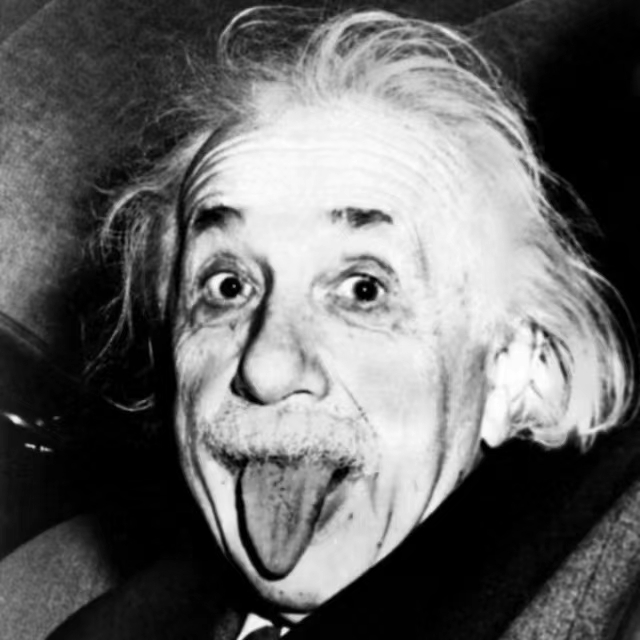
\includegraphics[width=2.8in]{Figures/mbti04-intp}% 
		\label{fig_text_feature_ablation}}
	\hfil
	\subfloat[]{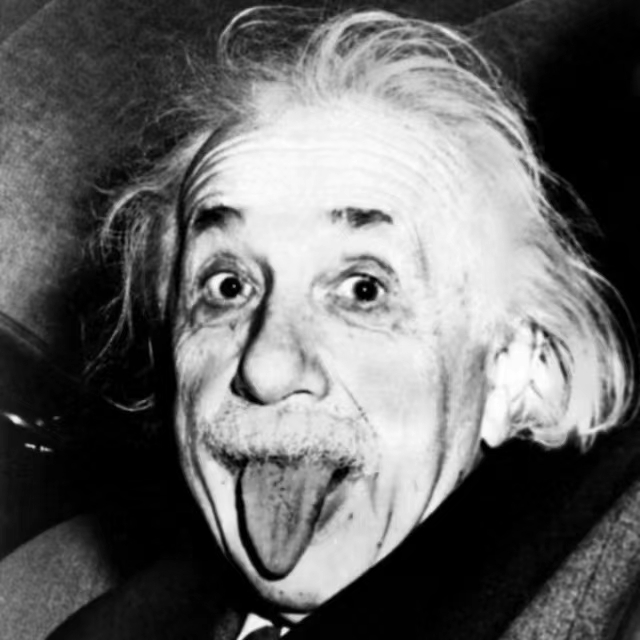
\includegraphics[width=2.8in]{Figures/mbti04-intp}
		\label{fig_visual_feature_ablation}}
	\bicaption{Lxx表现}{LMxxre ablation}
	\label{fig:feature ablation}
\end{figure*}


写点东西写点东西写点东西写点东西写点东西写点东西写点东西写点东西写点东西写点东西写点东西写点东西写点东西写点东西写点东西写点东西写点东西写点东西写点东西写点东西写点东西写点东西写点东西写点东西写点东西写点东西写点东西写点东西写点东西写点东西写点东西写点东西写点东西写点东西写点东西写点东西写点东西写点东西写点东西写点东西写点东西写点东西写点东西写点东西写点东西写点东西写点东西写点东西写点东西写点东西写点东西写点东西写点东西写点东西写点东西写点东西写点东西写点东西写点东西写点东西写点东西写点东西写点东西写点东西写点东西写点东西写点东西西写点东西写点东西写点东西写点东西写点东西写点东西写点东西写点东西写点东西写点东西写点东西写点东西写点东西写点东西写点东西写点东西写点东西写点东西写点东西写点东西写点东西写点东西写点东西写点东西写点东西写点东西写点东西写点东西写点东西写点东西写点东西写点东西写点东西写点东西写点东西写点东西写点东西写点东西写点东西写点东西写点东西写点东西写点东西写点东西写点东西写点东西写点东西写点东西写点东西写点东西写点东西写点东西写点东西写点东西写点东西写点东西写点东西写点东西写点东西写点东西写点东西写点东西写点东西写点东西写点东西写点东西写点东西写点东西写点东西写点东西写点东西写点东西写点东西写点东西写点东西点东西写点东西写点东西写点东西写点东西写点东西写点东西写点东西写点东西写点东西写点东西写点东西写点东西写点东西写点东西写点东西写点东西写点东西写点东西写点东西写点东西写点东西写点东西写点东西写点东西写点东西写点东西写点东西写点东西写点东西写点东西写点东西写点东西写点东西写点东西写点东西写点东西写点东西写点东西写点东西写点东西写点东西写点东西写点东西写点东西写点东西写点东西写点东西写点东西写点东西写点东西写点东西写点东西写点东西写点东西写点东西写点东西写点东西写点东西写点东西写点东西写点东西写点东西写点东西写点东西写点东西写点东西写点东西写点东西写点东西写点东西写点东西写点东西写点东西写点东西写点东西写点东西写点东西写点东西写点东西写点东西写点东西写点东西写点东西写点东西写点东西写点东西写点东西写点东西西写点东西写点东西写点东西写点东西写点东西写点东西写点东西写点东西写点东西写点东西写点东西写点东西写点东西写点东西写点东西写点东西写点东西写点东西写点东西写点东西写点东西写点东西写点东西写点东西写点东西写点东西写点东西写点东西写点东西写点东西写点东西写点东西写点东西写点东西写点东西写点东西写点东西写点东西写点东西写点东西写点东西写点东西写点东西写点东西写点东西写点东西写点东西写点东西写点东西写点东西写点东西写点东西写点东西写点东西写点东西写点东西写点东西写点东西写点东西写点东西写点东西写点东西写点东西写点东西写点东西写点东西写点东西写点东西写点东西写点东西写点东西写点东西写点东西写点东西写点东西点东西写点东西写点东西写点东西写点东西写点东西写点东西写点东西写点东西写点东西写点东西写点东西写点东西写点东西写点东西写点东西写点东西写点东西写点东西写点东西写点东西写点东西
写点东西写点东西写点东西写点东西写点东西写点东西写点东西写点东西写点东西写点东西写点东西写点东西写点东西写点东西写点东西写点东西写点东西写点东西写点东西写点东西写点东西写点东西写点东西写点东西写点东西写点东西写点东西写点东西写点东西写点东西写点东西写点东西写点东西写点东西写点东西写点东西写点东西写点东西写点东西写点东西写点东西写点东西写点东西写点东西写点东西写点东西写点东西写点东西写点东西写点东西写点东西写点东西写点东西写点东西写点东西写点东西写点东西写点东西写点东西写点东西写点东西写点东西写点东西写点东西写点东西写点东西写点东西西写点东西写点东西写点东西写点东西写点东西写点东西写点东西写点东西写点东西写点东西写点东西写点东西写点东西写点东西写点东西写点东西写点东西写点东西写点东西写点东西写点东西写点东西写点东西写点东西写点东西写点东西写点东西写点东西写点东西写点东西写点东西写点东西写点东西写点东西写点东西写点东西写点东西写点东西写点东西写点东西写点东西写点东西写点东西写点东西写点东西写点东西写点东西写点东西写点东西写点东西写点东西写点东西写点东西写点东西写点东西写点东西写点东西写点东西写点东西写点东西写点东西写点东西写点东西写点东西写点东西写点东西写点东西写点东西写点东西写点东西写点东西写点东西写点东西写点东西写点东西点东西写点东西写点东西写点东西写点东西写点东西写点东西写点东西写点东西写点东西写点东西写点东西写点东西写点东西写点东西写点东西写点东西写点东西写点东西写点东西写点东西写点东西





\vspace{12pt}
\begin{footnotesize}
	\begin{longtable}{|>{\columncolor{gray!15}}m{4cm}|m{1.7cm}<{\centering}|m{1.7cm}<{\centering}|m{1.7cm}<{\centering}|m{1.7cm}<{\centering}|}
		\bicaption{Top-3模xxTI对比}{Top-xxxtrue xxes}
		\label{fig:mbti case study}\\
		
		%表头
		\hline
		\endfirsthead
		

		% 表底
		\hline%\thickhline
		\endfoot
		
		\hline%\thickhline
		\endlastfoot
		
		% 第二组
		\hline\rowcolor{gray!15}
		\textbf{测试场景一} & \multicolumn{4}{c|}{\textbf{xxx}} \\ \hline
		\specialrule{0.75pt}{1pt}{0.5pt}\diagbox[dir=SE, width=4.4cm]{\textbf{xx}}{\textbf{xx}} & \raisebox{-.1\height}{\hspace{-1.5mm}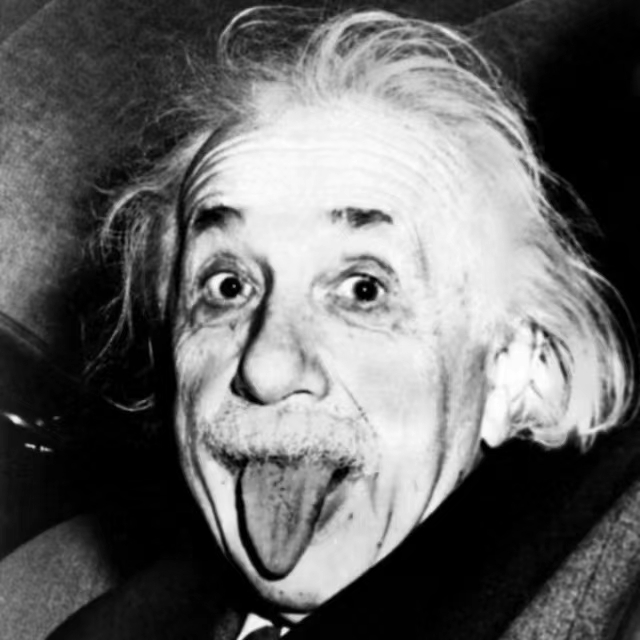
\includegraphics[width=2cm, keepaspectratio]{Figures/mbti04-intp}} & \raisebox{-.1\height}{\hspace{-1.5mm}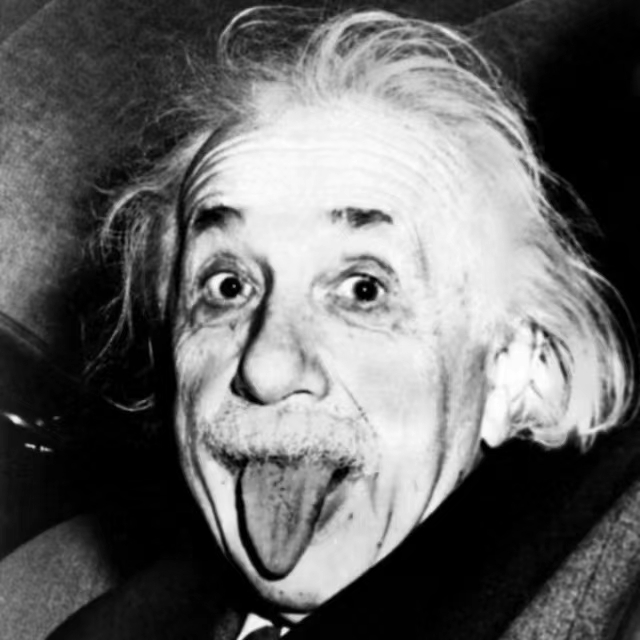
\includegraphics[width=2cm, keepaspectratio]{Figures/mbti04-intp}} & \raisebox{-.1\height}{\hspace{-1.5mm}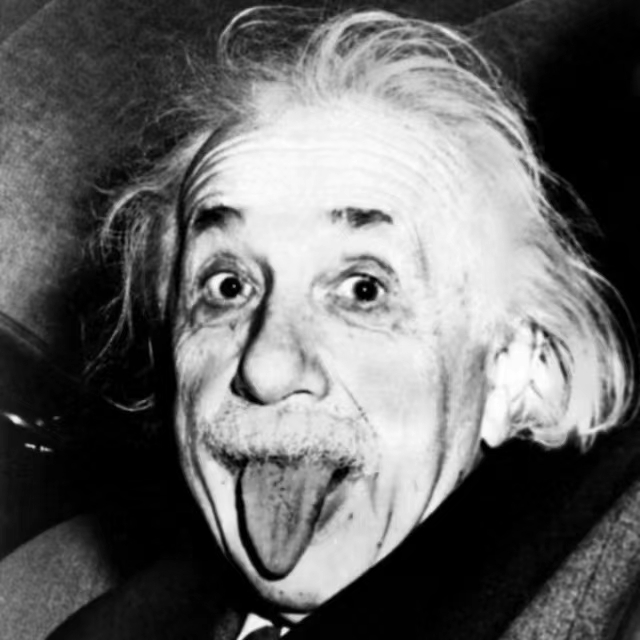
\includegraphics[width=2cm, keepaspectratio]{Figures/mbti04-intp}} & \raisebox{-.1\height}{\hspace{-1.5mm}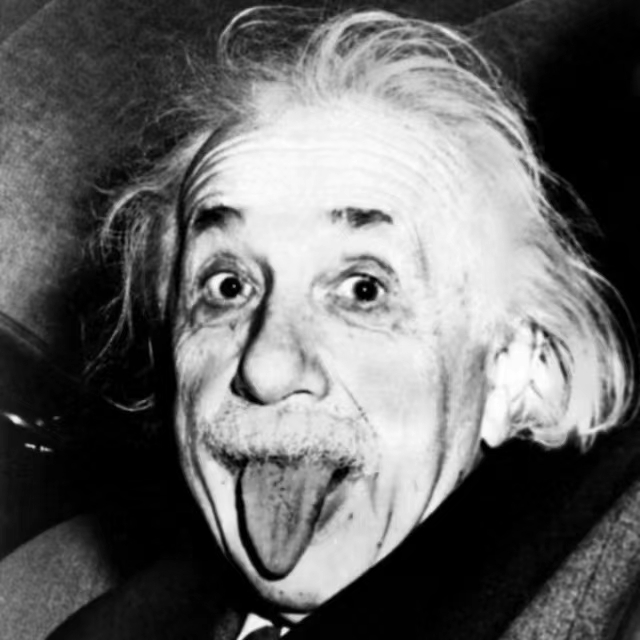
\includegraphics[width=2cm, keepaspectratio]{Figures/mbti04-intp}} \\
		\hline
		\specialrule{0.75pt}{1pt}{0.5pt}\cellcolor{white}\textbf{xxx} & \textbf{INFP} & \textbf{ENFP} & \textbf{ESTP} & \textbf{INTJ} \\
		\hline
		\cellcolor{white}xxx(ResNet Feature)
		& INF\textcolor{red}{J} & ENFP & E\textcolor{red}{N}TP & INTJ \\
		\hline
		\cellcolor{white}PM-xxx\cite{conferencekey} & INFP & ENFP & \textcolor{red}{IN}TP & I\textcolor{red}{S}TJ \\
		\hline
		\cellcolor{white}xxx\cite{conferencekey} & INF\textcolor{red}{J} & E\textcolor{red}{S}FP & E\textcolor{red}{N}T\textcolor{red}{J} & I\textcolor{red}{S}TJ \\
		\hhline{*{5}{:=}:}
		% 第三组
		\hline\rowcolor{gray!15}
		\textbf{测试场景二} & \multicolumn{4}{c|}{\textbf{单x拍}} \\ \hline
		\specialrule{0.75pt}{1pt}{0.5pt}\diagbox[dir=SE, width=4.4cm]{\textbf{测试模型}}{\textbf{xx}} & \raisebox{-.1\height}{\hspace{-1.5mm}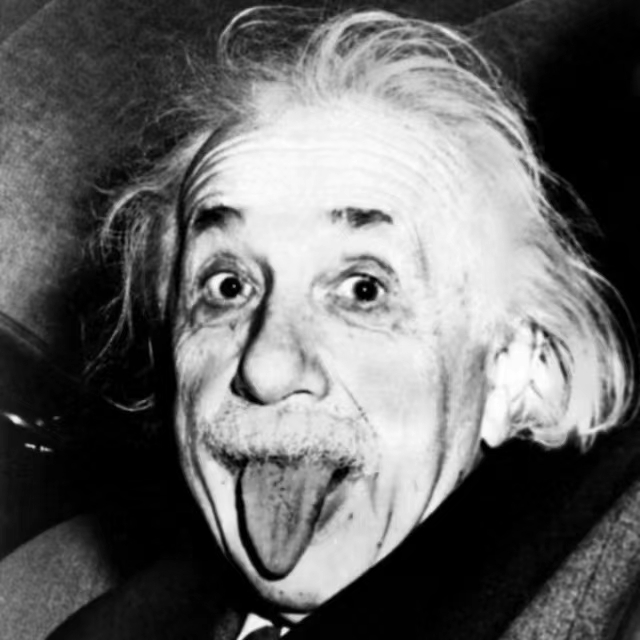
\includegraphics[width=2cm, keepaspectratio]{Figures/mbti04-intp}} & \raisebox{-.1\height}{\hspace{-1.5mm}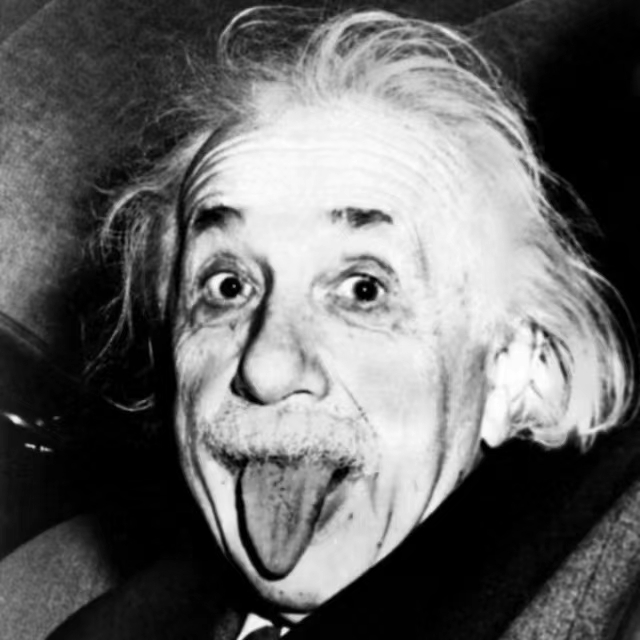
\includegraphics[width=2cm, keepaspectratio]{Figures/mbti04-intp}} & \raisebox{-.1\height}{\hspace{-1.5mm}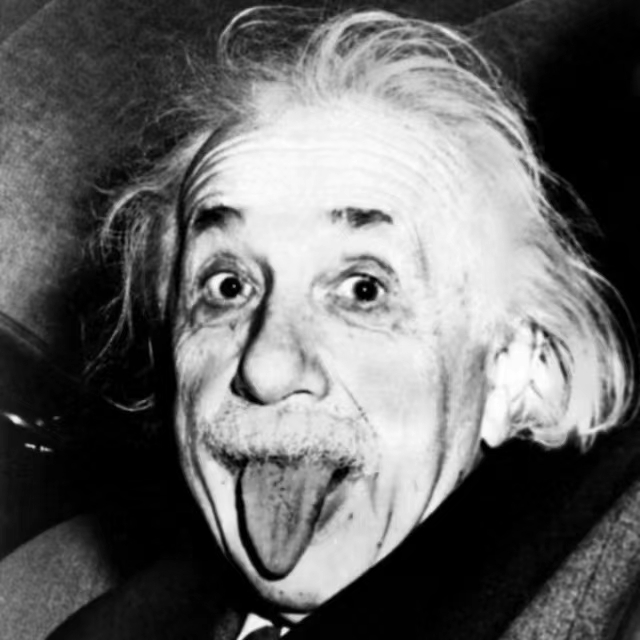
\includegraphics[width=2cm, keepaspectratio]{Figures/mbti04-intp}} & \raisebox{-.1\height}{\hspace{-1.5mm}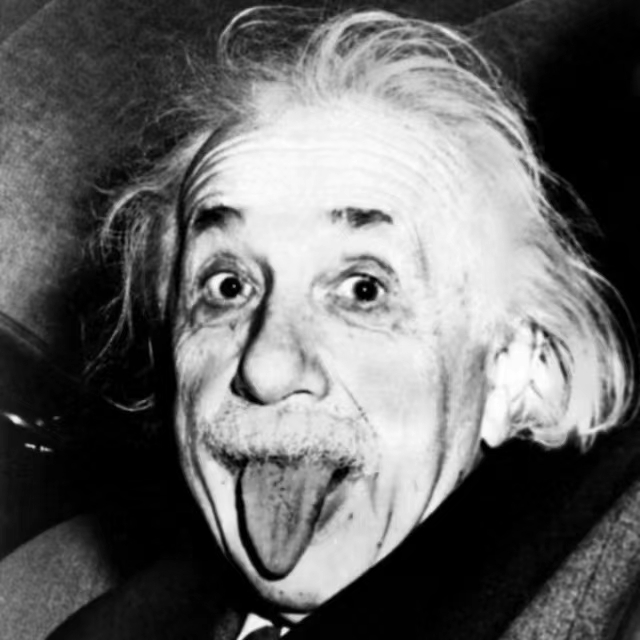
\includegraphics[width=2cm, keepaspectratio]{Figures/mbti04-intp}} \\
		\hline
		\specialrule{0.75pt}{1pt}{0.5pt}\cellcolor{white}\textbf{真实xTI} & \textbf{ISTJ} & \textbf{ISTJ} & \textbf{ISTJ} & \textbf{ISTJ} \\
		\hline
		\cellcolor{white}x(x Feature) & \textcolor{red}{ENF}J & \textcolor{red}{ENF}J & \textcolor{red}{E}S\textcolor{red}{F}J & \textcolor{red}{ENF}J \\
		\hline
		\cellcolor{white}PM-x\cite{conferencekey} & \textcolor{red}{ENF}J & \textcolor{red}{ENFP} & \textcolor{red}{E}S\textcolor{red}{FP} & I\textcolor{red}{NF}J \\
		\hline
		\cellcolor{white}xx\cite{conferencekey} & \textcolor{red}{ENFP} & \textcolor{red}{ENFP} & \textcolor{red}{ENF}J & \textcolor{red}{E}S\textcolor{red}{F}J \\
		%\hline
	\end{longtable}
\end{footnotesize}







\section{本章小结}

本章研究了x集。



	%!TEX root = ../Main.tex

\chapter{研究二}\label{ch-name2}
\section{引言}
xxx

\section{xxx}\label{sec-x x}
x描述:
\begin{equation}\begin{aligned}
	I &= M_{\text{idexy}}(\Theta_{\text{idxity}}) \\
	A &= M_{\text{xar}}(I, \Theta_{\text{xtar}}) \\
	B &= M_{\text{xxhy}}(I, \Theta_{\text{bixphy}}) \\
	\{T_1, T_2, \ldots, T_n\} &= M_{\text{twx}}(I, C, \Theta_{\text{txt}})
\end{aligned}\end{equation}
其中,\(\Theta_{\text{idexy}}\), \(\Theta_{\text{axr}}\), \(\Theta_{\text{bixhy}}\), 和 \(\Theta_{\text{txt}}\) 分别代表各模型的x征。


xxxx

\begin{table}[htbp]\footnotesize
	\centering
	
	\begin{threeparttable}[b]
		\bicaption{DPxx细信息}{Detailed infxx framework}
		\label{sec-llms}
		\begin{tabular}{@{}lllllll@{}}
			\hline%\toprule
			\rowcolor{gray!15}
			\textbf{机构} & \textbf{x} & \textbf{x} & \textbf{x} &  \textbf{x} & \textbf{x} & \textbf{x} \\ \hline%\midrule
			x           & Gxx-2\cite{journalkey}               & x-xl\tnote{1}  & 1.x              & Dec-x       & x & x\cite{journalkey}                   \\
			x      & Mistral\cite{conferencekey}              & x-7B-v0.1\tnote{2}  & x            & x-x       & N/A & x                   \\
			x      & LLaMA 2\cite{conferencekey}              & 
			x-2-x-x-hf\tnote{3}  & 7B           & Enc-Dec       & N/A & Mix                   \\
			x           & x-Neo\cite{conferencekey}              & x-x-2.7B\tnote{4}  & 2.x            & x-only       & N/A & Pile\cite{journalkey}                   \\
			x & x\cite{journalkey} & x-x\tnote{5} & 6B & Dec-only & GLM & Mix \\ 
			\hline%\bottomrule
		\end{tabular}%	
		
		\begin{tablenotes}
			\item[1] https://hxx-xl
			\item[2] https://xxistral-x
			\item[3] https://huxhf
			\item[4] https://huxx
			\item[5] https://hxnxx
		\end{tablenotes}
	\end{threeparttable}
\end{table}


\begin{table}[ht]\footnotesize
	\bicaption{TI-xx的性能表现}{TI-SAxataset}
	\label{tab:imxxtion}
	\centering
	\begin{threeparttable}[b]
		\begin{tabular}{>{\columncolor{gray!15}}m{4cm}||cc||ccc}
			\hline
			& \multicolumn{2}{c||}{\cellcolor{gray!15}\textbf{x}} & \multicolumn{3}{c}{\cellcolor{gray!15}\textbf{x(高亲和力)}} \\
			\cline{2-6}
			\multirowcell{-2}{\textbf{x}} & \cellcolor{gray!15}x$\downarrow$ & \cellcolor{gray!15}R-x(\%)$\uparrow$ &  \cellcolor{gray!15}x$\downarrow$ & \cellcolor{gray!15}R-x(\%)$\uparrow$ & \cellcolor{gray!15}P-x$\downarrow$\\
			\hline
			\cellcolor{white}\textbf{TI-x-x} & \underline{86.x} & \underline{92.17}  & \underline{93.74}  & \underline{89.13}  & \underline{26.x} \\
			\hline
			\cellcolor{white}w/o x w x & 138.54 & 75.16  & 146.37 & 71.15 & 47.51 \\
			\cellcolor{white}w/o x w FULL & 117.72 & 77.03  & 122.01 &  72.57 & 47.03  \\
			\hline
			\cellcolor{white}w/o x & \textbf{78.32} & \textbf{95.89}  & \textbf{83.46} & \textbf{93.42} &  44.39 \\
			\cellcolor{white}w/o x & 138x.69 & 74.98  & 139.60 & 71.42 &  \textbf{20.73} \\
			\hline
			\cellcolor{white}w/o x & 106.74 & 83.31  & 117.67 & 79.93 & 36.01 \\
			\cellcolor{white}w/o x & 88.06 & 90.72  & 97.32 & 87.05 & 29.10 \\
			\hline
		\end{tabular}
	\begin{tablenotes}
		\item[*] x,因此衡量P-x
	\end{tablenotes}
	\end{threeparttable}
\end{table}



\subsection{案例分析}

\subsubsection{x}

本文xx像(如图\ref{fig:avatar gen case study}(\subref{fig_female})和图\ref{fig:avatar gen case study}(\subref{fig_male}))和指xx性比较(如图\ref{fig:avatar gen case study}(\subref{fig_female_agreeable})和图\ref{fig:avatar gen case study}(\subref{fig_female_agreeable}))。
\vspace{12pt}
\begin{figure*}[!htbp]
	\centering
	\subfloat[]{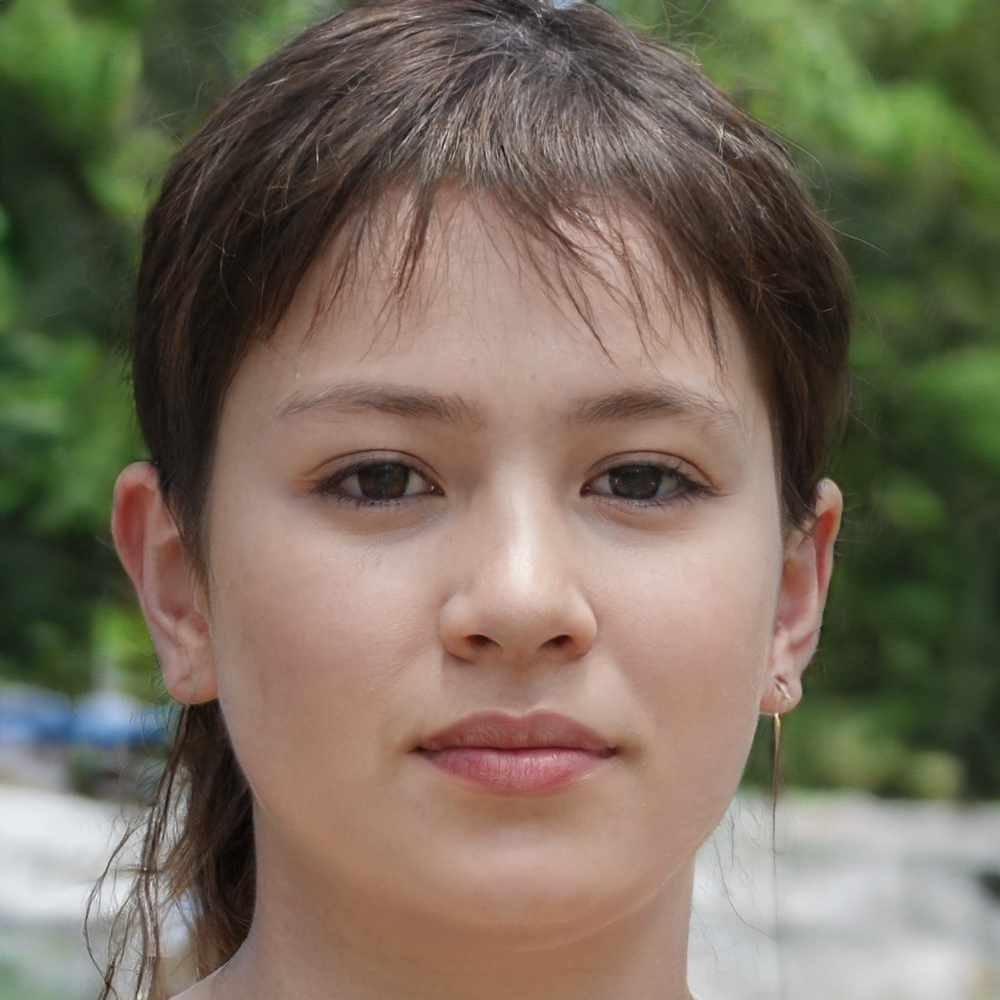
\includegraphics[width=1.8in]{Figures/sample-14}% 1.5
		\label{fig_female}}
	\hfil
	%	\hspace*{\fill}
	\subfloat[]{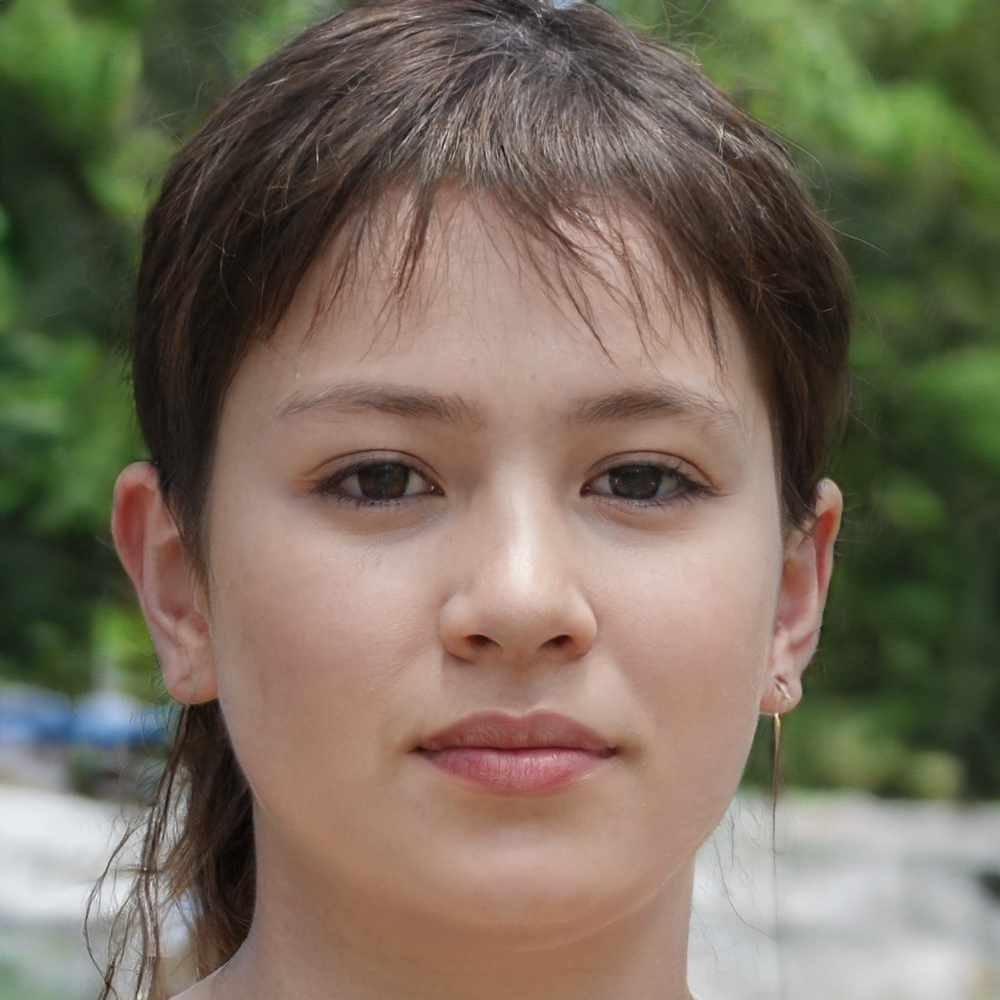
\includegraphics[width=1.8in]{Figures/sample-12}% 1.5
		\label{fig_female_agreeable}}
	\\ \vspace*{12pt}
	\subfloat[]{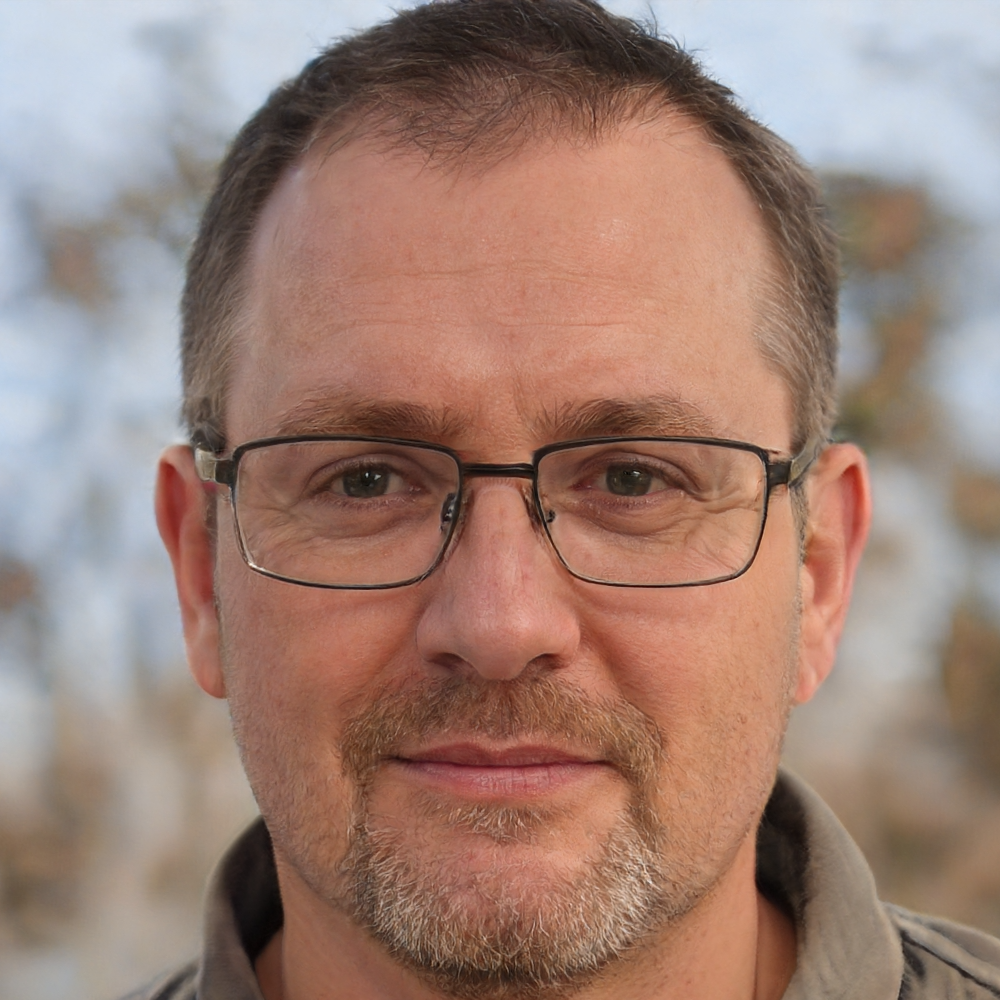
\includegraphics[width=1.8in]{Figures/sample-35}% 1.5
		\label{fig_male}}
	\hfil
	\subfloat[]{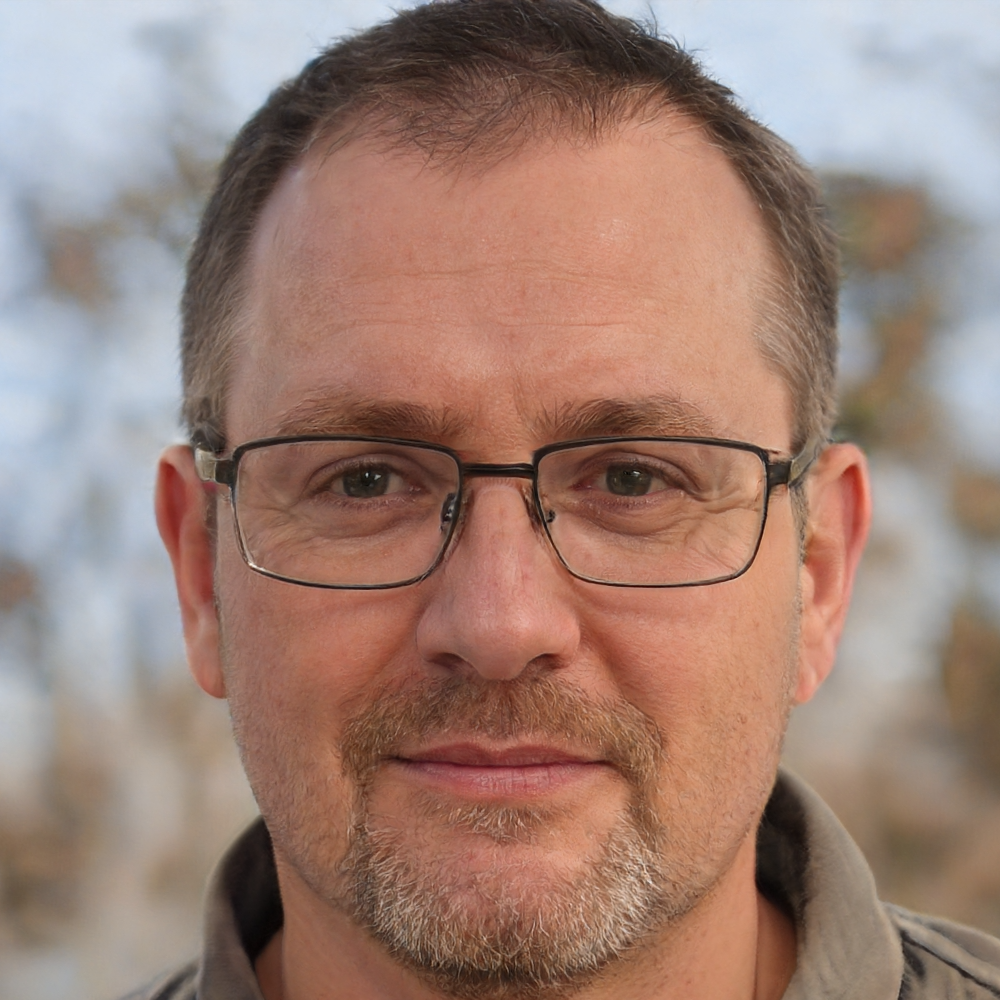
\includegraphics[width=1.8in]{Figures/sample-39}% 1.5
		\label{fig_male_agreeable}}
	\bicaption{不xx例}{Sampxxities}
	\label{fig:avatar gen case study}
\end{figure*}

x

\section{本章小结}
xx




	%!TEX root = ../Main.tex

\chapter{ 研究三}\label{ch-x}
\section{引言}
xx

\section{x}
\subsection{x}\label{sec-xx x}


\begin{table}[H]\footnotesize%[ht]\footnotesize
	\centering
	\begin{threeparttable}[b]

%	\caption{社xx准差}
	\bicaption{社交xxF1值}{Fxatasets}
	\label{tbl:adsfaf-detection}
	\begin{tabular}{lccccc}
		\hline
		\rowcolor{gray!15}
		方法 & 特征类型 & C-R-19\cite{conferencekey} & B-F-19\cite{conferencekey} & Twx0\cite{conferencekey} & Twx2\cite{conferencekey} \\
		\hline
		Dexot\cite{conferencekey} & 特xx本  & 51.2 ($\pm$0.0) & 77.0 ($\pm$0.0) & 73.1 ($\pm$0.0) & \underline{76.5} ($\pm$0.0) \\
		C-xM\cite{conferencekey} & 特x本  & 62.9 ($\pm$0.8) & \underline{74.0} ($\pm$4.7) & 59.6 ($\pm$0.7) & 65.9 ($\pm$0.0) \\
		MxM\cite{conferencekey} & x本  & / & / & 71.3 ($\pm$1.6) & 70.2 ($\pm$1.2) \\
		RxExa\cite{conferencekey} & x本  & / & / & 75.5 ($\pm$0.1) & 72.1 ($\pm$0.1) \\
		Tx\cite{conferencekey} & 文本  & / & / & 73.5 ($\pm$0.1) & 72.1 ($\pm$0.1) \\
		LxO\cite{conferencekey} & xxx本  & / & / & 77.4 ($\pm$0.2) & 75.7 ($\pm$0.1) \\
		\hline
	\end{tabular}
	\begin{tablenotes}
		\item[*] ``/''表示数据x应的模型。
	\end{tablenotes}
	\end{threeparttable}
\end{table}

嘻嘻嘻嘻

\begin{table}[htbp]\footnotesize
	\centering
	\bicaption{社x卷}{Sociaxuestionnaire}
	\label{tbl:trust survey}
	\begin{tabular}{|c|l|c|}
		\hline
		\rowcolor{gray!15}
		\multicolumn{3}{|l|}{\textbf{背}} \\
		\hline
		\multicolumn{3}{|p{14cm}|}{假设12324243424jifjoj9q9r8u0ufjfe0jfaeoua98ur9f9ebfcaeybfcyae87rca87fcasycacyfa7yc8ysy联系。} \\
		\hhline{*{3}{:=}:}
		\rowcolor{gray!15}
		\textbf{编x} & \;\;\,\textbf{问x述} & \textbf{选x} \\
		\hline
		Q1 & \;\;\,该用x确 & \begin{tabular}{l} 
			0\%(强x意), 10\%, 20\%, 30\%, 40\% \\
			50\%(不x), 60\%, 70\%, 80\%, 90\%, 100\%
		\end{tabular} \\
		\hline
		Q2 & \;\;\,该x知识 &  同Q1 \\
		\hline
		Q3 & \;\;\,此人xx欢迎 & 同Q1  \\
		\hline
		Q4 & \begin{tabular}{l} 
			该x些信息(如x介、\\x文等)  
			影响了x
		\end{tabular} 
		& [文x框] \\
		\hline
		Q5 & \;\;\,你是x择x该x户 & x注 / 忽x略 \\
		\hline
	\end{tabular}
\end{table}





\section{本章小结}

本章研究了xx。





	%!TEX root = ../Main.tex

\chapter{总结与展望}
\section{主要工作总结}
随着x具有重大理论和实践意义。

本文主要研究了x进行了评估。

本文的研究工作主要包括以下三点:

\textbf{(1)社x究}

首先x


\textbf{(2)人x研究}

首先x



\textbf{(3)社x研究}

为了x

\section{未来工作展望}

本文探索了x,未来研究可从以下方面展开:

\textbf{(1)探x方法}

目前,x。



\textbf{(2)研究x法}

本文为x。

\textbf{(3)优化x方案}

本文的x


\textbf{(4)探究x策略}

在未来的研x
	
	% 设置论文正文后的式样
	\backmatter
	% 按国标自动制作参考文献
	% 参考文献数据文件为本目录下的Reference.bib
	\begin{reference}
		\bibliographystyle{gbt7714-numerical}
		\bibliography{Reference}
	\end{reference}
	% 包含在读期间科研成果
	%!TEX root = ../Main.tex

% 作者在读期间科研成果简介
\chapter{攻读学位期间科研及成果简介}  % 攻读学位期间取得的研究成果
%\section*{发表论文}
%\emph{(暂无)}
%\section*{承担科研项目}
%\emph{(暂无)}

\noindent\textbf{(一)作者发表的学术论文情况}
\vspace{0.25em}

\noindent[1] First Name Last Name, First Name Last Name, First Name Last Name. Paper Title [J]. \textit{Expert Systems with Applications}, 202x, 2x7: 11xx38.(中科院1区期刊,已正式发表,本人第一作者)

\noindent[2] First Name Last Name, First Name Last Name, First Name Last Name. Paper Title [J]. \textit{IEEE Transactions on Information Forensics and Security}, 2024.(CCF-A期刊,第二轮评审中,本人第一作者)

\noindent[3]x. x [J]. \textit{IEEE Transactions on Knowledge and Data Engineering}, 2024.(CCF-A期刊,已投稿,本人第三作者)

\vspace{1em}

\noindent\textbf{(二)作者申请的专利情况}
\vspace{0.25em}

\noindent[1] 中文名字,中文名字,中文名字,中文名字,中文名字,中文名字,中文名字. 一种x方法[P]. 中国专利,申请专利号:ZL 20x5.7,申请时间:202x-0x-02. (实审中,本人第二发明人,导师第一发明人)

\noindent[2] 中文名字,中文名字,中文名字,中文名字,中文名字,中文名字,中文名字. 基于多x方法[P]. 中国专利,专利号:ZL x.6,申请时间:202x-09-x2. (实审中,本人第三发明人)

\noindent[3] 中文名字,中文名字,中文名字,中文名字,中文名字,中文名字,中文名字. 一种基于x方法[P]. 中国专利,专利号:ZL 202x71266.1 授权时间:202x-07-0x.(已正式授权,本人第六发明人)

\vspace{1em}

\noindent\textbf{(三)研究生阶段参与的项目与课题}
\vspace{0.25em}

\noindent[1] 国家重x题,项目名称:智xx会x多x及实x系模型,项目编号:202xFx3101-2,起止日期:202x.1x-202x.0x,纵向项目,在研,参与.


\noindent[2] 四川x划项目,项目名称:面向网x协x技术研究,项目编号:202xG0145,起止日期:202x.1-202x.12,纵向项目,在研,参与.


\noindent[3] 教育部x项目,项目名称:网络x及应x研究,项目编号:CMx409,起止日期:202x.1-202x.12,纵向项目,已结题,参与.





	%\makethanks
	% 包含致谢
	%!TEX root = ../Main.tex

% 致谢 
\makechaptertitlecenter\chapter{致\hspace{1em}谢}
好好写吧
	
	

	%\makestatement
	% 包含论文原创性声明(请勿修改)
	%!TEX root = ../Main.tex


% 原创性声明
\chapter{声\hspace{1em}明}
本人声明所呈交的学位论文是本人在导师指导下进行的研究工作及取得的研究成果。据我所知,除了文中特别加以标注和致谢的地方外,论文中不包含其他人已经发表或撰写过的研究成果,也不包含为获得四川大学或其他教育机构的学位或证书而使用过的材料。与我一同工作的同志对本研究所做的任何贡献均已在论文中作了明确的说明并表示谢意。


本学位论文成果是本人在四川大学读书期间在导师指导下取得的,论文成果归四川大学所有,特此声明。
\vspace{4cm}
\autograph

	% 包含论文版权授权书(请勿修改)
	%!TEX root = ../Manual.tex
\chapter{学位论文版权使用授权书}
本学位论文作者完全了解\universityname有关保留、使用学位论文的规定,有权保留并向国家有关部门或机构送交论文的复印件和磁盘,允许论文被查阅和借阅。本人授权\universityname可以将学位论文的全部或部分内容编入有关数据库进行检索,可以采用影印、缩印或扫描等复制手段保持、汇编学位论文。


(保密的学位论文在解密后适用本授权书)
\vspace{4cm}
\autograph

\end{document}
